% Options for packages loaded elsewhere
\PassOptionsToPackage{unicode}{hyperref}
\PassOptionsToPackage{hyphens}{url}
%
\documentclass[
  english,
  man]{apa6}
\usepackage{lmodern}
\usepackage{amssymb,amsmath}
\usepackage{ifxetex,ifluatex}
\ifnum 0\ifxetex 1\fi\ifluatex 1\fi=0 % if pdftex
  \usepackage[T1]{fontenc}
  \usepackage[utf8]{inputenc}
  \usepackage{textcomp} % provide euro and other symbols
\else % if luatex or xetex
  \usepackage{unicode-math}
  \defaultfontfeatures{Scale=MatchLowercase}
  \defaultfontfeatures[\rmfamily]{Ligatures=TeX,Scale=1}
\fi
% Use upquote if available, for straight quotes in verbatim environments
\IfFileExists{upquote.sty}{\usepackage{upquote}}{}
\IfFileExists{microtype.sty}{% use microtype if available
  \usepackage[]{microtype}
  \UseMicrotypeSet[protrusion]{basicmath} % disable protrusion for tt fonts
}{}
\makeatletter
\@ifundefined{KOMAClassName}{% if non-KOMA class
  \IfFileExists{parskip.sty}{%
    \usepackage{parskip}
  }{% else
    \setlength{\parindent}{0pt}
    \setlength{\parskip}{6pt plus 2pt minus 1pt}}
}{% if KOMA class
  \KOMAoptions{parskip=half}}
\makeatother
\usepackage{xcolor}
\IfFileExists{xurl.sty}{\usepackage{xurl}}{} % add URL line breaks if available
\IfFileExists{bookmark.sty}{\usepackage{bookmark}}{\usepackage{hyperref}}
\hypersetup{
  pdftitle={National Longitudinal Study Reveals Growth in Wellbeing Among Those with Spiritual Beliefs},
  pdfauthor={Ben Highland1, Everett L. Worthington2, Don E Davis3, Chris G. Sibley4, \& Joseph Bulbulia5},
  pdflang={en-EN},
  pdfkeywords={Belief, God, Health, Longitudinal, Panel, Religion, Spirit, Spirituality, Well-being},
  hidelinks,
  pdfcreator={LaTeX via pandoc}}
\urlstyle{same} % disable monospaced font for URLs
\usepackage{graphicx,grffile}
\makeatletter
\def\maxwidth{\ifdim\Gin@nat@width>\linewidth\linewidth\else\Gin@nat@width\fi}
\def\maxheight{\ifdim\Gin@nat@height>\textheight\textheight\else\Gin@nat@height\fi}
\makeatother
% Scale images if necessary, so that they will not overflow the page
% margins by default, and it is still possible to overwrite the defaults
% using explicit options in \includegraphics[width, height, ...]{}
\setkeys{Gin}{width=\maxwidth,height=\maxheight,keepaspectratio}
% Set default figure placement to htbp
\makeatletter
\def\fps@figure{htbp}
\makeatother
\setlength{\emergencystretch}{3em} % prevent overfull lines
\providecommand{\tightlist}{%
  \setlength{\itemsep}{0pt}\setlength{\parskip}{0pt}}
\setcounter{secnumdepth}{-\maxdimen} % remove section numbering
% Make \paragraph and \subparagraph free-standing
\ifx\paragraph\undefined\else
  \let\oldparagraph\paragraph
  \renewcommand{\paragraph}[1]{\oldparagraph{#1}\mbox{}}
\fi
\ifx\subparagraph\undefined\else
  \let\oldsubparagraph\subparagraph
  \renewcommand{\subparagraph}[1]{\oldsubparagraph{#1}\mbox{}}
\fi
% Manuscript styling
\usepackage{upgreek}
\captionsetup{font=singlespacing,justification=justified}

% Table formatting
\usepackage{longtable}
\usepackage{lscape}
% \usepackage[counterclockwise]{rotating}   % Landscape page setup for large tables
\usepackage{multirow}		% Table styling
\usepackage{tabularx}		% Control Column width
\usepackage[flushleft]{threeparttable}	% Allows for three part tables with a specified notes section
\usepackage{threeparttablex}            % Lets threeparttable work with longtable

% Create new environments so endfloat can handle them
% \newenvironment{ltable}
%   {\begin{landscape}\begin{center}\begin{threeparttable}}
%   {\end{threeparttable}\end{center}\end{landscape}}
\newenvironment{lltable}{\begin{landscape}\begin{center}\begin{ThreePartTable}}{\end{ThreePartTable}\end{center}\end{landscape}}

% Enables adjusting longtable caption width to table width
% Solution found at http://golatex.de/longtable-mit-caption-so-breit-wie-die-tabelle-t15767.html
\makeatletter
\newcommand\LastLTentrywidth{1em}
\newlength\longtablewidth
\setlength{\longtablewidth}{1in}
\newcommand{\getlongtablewidth}{\begingroup \ifcsname LT@\roman{LT@tables}\endcsname \global\longtablewidth=0pt \renewcommand{\LT@entry}[2]{\global\advance\longtablewidth by ##2\relax\gdef\LastLTentrywidth{##2}}\@nameuse{LT@\roman{LT@tables}} \fi \endgroup}

% \setlength{\parindent}{0.5in}
% \setlength{\parskip}{0pt plus 0pt minus 0pt}

% \usepackage{etoolbox}
\makeatletter
\patchcmd{\HyOrg@maketitle}
  {\section{\normalfont\normalsize\abstractname}}
  {\section*{\normalfont\normalsize\abstractname}}
  {}{\typeout{Failed to patch abstract.}}
\patchcmd{\HyOrg@maketitle}
  {\section{\protect\normalfont{\@title}}}
  {\section*{\protect\normalfont{\@title}}}
  {}{\typeout{Failed to patch title.}}
\makeatother
\shorttitle{Beliefs and Wellbeing}
\keywords{Belief, God, Health, Longitudinal, Panel, Religion, Spirit, Spirituality, Well-being\newline\indent Word count: 4778}
\DeclareDelayedFloatFlavor{ThreePartTable}{table}
\DeclareDelayedFloatFlavor{lltable}{table}
\DeclareDelayedFloatFlavor*{longtable}{table}
\makeatletter
\renewcommand{\efloat@iwrite}[1]{\immediate\expandafter\protected@write\csname efloat@post#1\endcsname{}}
\makeatother
\usepackage{csquotes}
\usepackage{tcolorbox}
\usepackage{paralist}
\usepackage{multicol}
\usepackage{graphics}
\usepackage{rotating}
\usepackage{longtable}
\ifxetex
  % Load polyglossia as late as possible: uses bidi with RTL langages (e.g. Hebrew, Arabic)
  \usepackage{polyglossia}
  \setmainlanguage[]{english}
\else
  \usepackage[shorthands=off,main=english]{babel}
\fi

\title{National Longitudinal Study Reveals Growth in Wellbeing Among Those with Spiritual Beliefs}
\author{Ben Highland\textsuperscript{1}, Everett L. Worthington\textsuperscript{2}, Don E Davis\textsuperscript{3}, Chris G. Sibley\textsuperscript{4}, \& Joseph Bulbulia\textsuperscript{5}}
\date{}


\authornote{

1 Wake Forest Medical School 2 Department of Psychology Virginia Commonwealth University 3 Department of Psychology Georgia State University 4 School of Psychology University of Auckland 5 School of Psychology Victoria University

}

\affiliation{\phantom{0}}

\abstract{
Previous research finds an association between spirituality and subjective well-being. However, the widespread use of tautological spirituality scales, poorly defined concepts of spirituality, and reliance on cross-sectional samples cast doubts. Here, we leverage nine years of panel data from a nationally diverse longitudinal study to systematically test whether having spiritual beliefs leads to growth in personal well-being and life satisfaction (\(N\) = 20979, New Zealand, 2010-2018). Contrary to previous research, we find that belief in a spirit or life force predicts lower personal well-being and life-satisfaction. However, in support of previous speculation, beliefs in a spirit or life force predict increasing personal well-being and life satisfaction over time relative to disbelief. These finding holds after adjusting for known demographic influences, and intriguingly, among those who believe in a God but disbelieve in a spirit or life force. The recent growth in spiritual beliefs and decline in traditional religion across many industrial societies motivates further causal investigations of the social and psychological mechanisms through which spiritual beliefs lead to growth in subjective well-being.
}



\begin{document}
\maketitle

The relationship between spirituality and psychological well-being is a matter of enduring fascination (Ellsworth \& Ellsworth, 2010). Most previous attempts to quantify the relationship between these two domains find a positive association: spirituality predicts well-being (Ginsburg, Quirt, Ginsburg, \& MacKillop, 1995; Koenig, 2010; Koenig, Associate Professor of Psychology and Religious Studies Michael E McCullough, PhD, McCullough, Larson, \& Adjunct Professor of Psychiatry David B Larson, 2001; Russinova, Wewiorski, \& Cash, 2002; Smith, McCullough, \& Poll, 2003; Smith et al., 2003; Zaza, Sellick, \& Hillier, 2005). However, critics raise three challenges.

First, previous research has frequently operationalised spirituality using measures of well-being. For example, The Daily Spiritual Experience Scale, which is widely used in spiritual mental health research, includes items such as \enquote{I feel thankful for my blessings} and \enquote{I feel deep inner peace or harmony} to measure spirituality (Underwood \& Teresi, 2002). As Koenig observes, it is unsurprising that spirituality predict well-being when the same items are used to measure both constructs. Koenig aptly describes this features as a \enquote{tautology} in spirituality/mental health research (Koenig, 2008). Indeed, recent systematic-review of spirituality/mental health research found that nearly 45\% of previous studies employe tautological scales (Garssen et al., 2016). The first challenge, then, is to define measures of spirituality that are not well-being measures dressed in other words.

A second challenge is to disentangle concepts of spirituality from concepts of religion. The term \enquote{spirituality} was first used to describe the religious practices of ascetics and monks, however, more recently, the term has taken on a broader family of meanings (Swinton, 2001). However previous research does not converge on a unique set of meanings. Most studies of spirituality and religion have been conducted among (cross-sectional) North American samples among people who are affiliate with traditional religion (Ano \& Vasconcelles, 2005; Hackney \& Sanders, 2003; Sawatzky, Ratner, \& Chiu, 2005; Smith et al., 2003; Visser, Garssen, \& Vingerhoets, 2010; Yonker, Schnabelrauch, \& Dehaan, 2012). However, when spirituality has been operationalised as distinct from religion, some researchers have found a negative association within subjective well-being (King et al., 2013). Thus, in addition to disentangling the concept of spirituality from concepts of subjective well-being, it is also important to disentangle the concept of spirituality from concepts of religion.

A third challenge is to investigate the relationship between spirituality and subjective well-being over the life-span in nationally diverse samples. To assess whether spiritual beliefs lead to growth, stability, or decline in psychological well-being requires comparing requires repeatedly measuring individuals who differ in spirituality, demography, and religion as these people age, and investigating how their perceive their lives to be turning out (Garssen \& Visser, 2016). However, previous investigations of spirituality and well-being, including high-quality reviews and meta-analyses, have relied on cross-sectional samples (Ano \& Vasconcelles, 2005; Hackney \& Sanders, 2003; Sawatzky et al., 2005; Smith et al., 2003; Visser et al., 2010; Yonker et al., 2012). To address the key questions in spirituality psychological health research, then, requires longitudinal investigations.

Here, we addresses the three challenges of previous in the following ways: First, to avoid a tautological elision of \enquote{spirituality} and \enquote{well-being} we adopt a non-affective measure of spirituality as a \enquote{believe in a Spirit or Life Force.} On the other side, to measure subjective well-being, we use a well-validated scale for Personal Well-being and a well-validated scale for Life-Satisfaction (see Method). Second, to disentangle spiritual beliefs from traditional religious beliefs and skeptical beliefs we adopt a four-level categorical indicator combining the binary indicator of belief in a Spirit or Life Force with the binary indicator \enquote{Do you believe in some form of a spirit or life force?} The levels of this four-level categorical indicator for spiritual, religious, and skeptical beliefs are as follows: (1) Skeptics: those who neither believe in a God nor believe in a Spirit or Life force; (2) Skeptics about God who nevertheless believe in a Spirit or Life Force; (3) Those who believe in a God but do not believe in a Spirit or Life force; (4) Those who who believe in a both God and a Spirit or Life Force. Clearly such an approach cannot simultaneously address all interests in previous spirituality/well-being research. For example we do not combine our cognitive measure of belief with behavioral measures or attitudinal measures. However, this cost to scope is paid for with benefits to precision. The spiritual indicators measure cognitive states in which distinct varieties of skeptical beliefs, traditional religious beliefs, and non-traditional spirit beliefs are straightforwardly disentangled, and measured within people. Third, to assess whether spirit beliefs lead to growth, stability, or decline in psychological well-being, we leverage longitudinal responses from a nationally diverse probability sample year over an nine--year period with nine measurement points (2010 to 2018 New Zealand Attitudes and Values Study, NZAVS).

\hypertarget{method}{%
\section{Method}\label{method}}

The New Zealand Attitudes and Values Study (NZAVS) is reviewed every three years by the University of Auckland Human Participants Ethics Committee. Our most recent ethics approval statement is as follows: The New Zealand Attitudes and Values Study was approved by The University of Auckland Human Participants Ethics Committee on 03-June-2015 until 03-June-2018, and renewed on 05-September-2017 until 03-June-2021. Reference Number: 014889. Our previous ethics approval statement for the 2009-2015 period is: The New Zealand Attitudes and Values Study was approved by The University of Auckland Human Participants Ethics Committee on 09-September-2009 until 09-September-2012, and renewed on 17-February-2012 until 09-September-2015. Reference Number: 6171. All participants granted informed written consent and The University of Auckland Human Participants Ethics Committee approved all procedures.

\hypertarget{sampling-procedure}{%
\subsection{Sampling Procedure}\label{sampling-procedure}}

The NZAVS is an annual, longitudinal national probability sample of registered New Zealand voters, which was started in 2009. The Time 10 wave of the NZAVS contained responses from 47,951 participants (17,981 retained from one or more previous waves and 29,970 new additions from booster sampling and/or unmatched participants or unsolicited opt-ins). Participants who provided an email address were also emailed and invited to complete an online version if they preferred. We offered a prize draw for participation, non-respondents were emailed and phoned multiple times, and all participants were mailed a Season's Greetings card from the NZAVS research team and informed that they had been automatically entered into a bonus seasonal grocery voucher prize draw. We also mailed our yearly pamphlet summarizing key research findings published during the current wave of the study.

\hypertarget{participants}{%
\subsection{Participants}\label{participants}}

The Time 10 (2018) wave of the NZAVS included 47,951 respondents. We analyzed data from participants who responded to our survey at least three four times between Time 2 (2010) and Time 10 (2018), resulting in a sample of N = 21,705 (N = 20,979 with complete responses).

\hypertarget{measures}{%
\subsection{Measures}\label{measures}}

\textbf{Life Satisfaction} Life satisfaction is a measure of emotional well-being that was assessed using a 2-item version of the Satisfaction With Life Scale, which has previously been shown to correlate with aspects of religiosity (Diener, Emmons, Larsen, \& Griffin, 1985). Participants rated their agreement with the statements (a) \enquote{I am satisfied with my life}; and (b) \enquote{In most ways my life is close to ideal.} The items were rated on 7-point response options ranging from 1 = strongly disagree to 7 = strongly agree. The mean Cronbach's alpha for this 2-item scale was \(\alpha\) = 0.90. Higher scores on this scale indicate higher life satisfaction. Overall scores were means of the 2-items. For detailed information pertaining to means, standard deviations, and missingness, see Table 1.

\textbf{Personal well-being} Personal well-being is a measure of function all well-being that was assessed using a 4-item version of the Australian Unity well-being Index (Cummins, Eckerseley, Pallant, Van Vugt, \& Misajon, 2017). Participants rated their satisfaction with (a) \enquote{Your standard of living}; (b) \enquote{Your health}; (c) \enquote{Your future security}; (d) \enquote{Your personal relationships.} Items were rated using a 10-point response option ranging from 1 = completely dissatisfied to 10 = completely satisfied. The mean Cronbach's alpha for this scale was \(\alpha\) = 0.90. Higher scores on this scale indicate higher personal well-being. Overall scores were means of the 4-items. For detailed information pertaining to means, standard deviations, and missingness, see Table 1.

\textbf{\emph{Belief in a Spirit or a God}} We assess belief in a spirit or a God by asking two non-affective questions: \enquote{Do you believe in a spirit or life force} and \enquote{Do you believe in a god?} Responses were coded as (1) Skeptics: those who neither believe in a God nor believe in a Spirit or Life force; (2) Skeptics about God who believe in a Spirit or Life Force; (3) Believers in a God who disbelieve in a Spirit or Life force; (4) Believers in a God and Spirit or Life Force. These believe were developed for the NZAVS from the 2005 Eurobarometer. For detailed information pertaining to beliefs, see Table 1.

Table 1 about here:
\[
\begin{table}[ ht ] 
\centering 
\caption{}\label{}
\scalebox{.6}{
\begin{tabular}{ l c c c c c c c c c }
\toprule
 &   \multicolumn{ 9 }{c}{ Wave }\\ 
  & 2010 & 2011 & 2012 & 2013 & 2014 & 2015 & 2016 & 2017 & 2018 \\ 
 & n = \emph{missing} & n = \emph{missing} & n = 8547 & n = 13472 & n = \emph{missing} & n = 11687 & n = 16048 & n = 14174 & n = 14883 \\ 
 \midrule
Age &   &   &   &   &   &   &   &   &  \\ 
NZdep &   &   &   &   &   &   &   &   &  \\ 
Education &   &   &   &   &   &   &   &   &  \\ 
Employed &   &   &   &   &   &   &   &   &  \\ 
\hspace{6pt}    0 &  (\%) &  (\%) & 2094 (24.5\%) & 2955 (21.9\%) &  (\%) & 2525 (21.6\%) & 3486 (21.7\%) & 3223 (22.7\%) & 3404 (22.9\%)\\ 
\hspace{6pt}    1 &  (\%) &  (\%) & 6453 (75.5\%) & 10517 (78.1\%) &  (\%) & 9162 (78.4\%) & 12562 (78.3\%) & 10951 (77.3\%) & 11479 (77.1\%)\\ 
EthnicCategories &   &   &   &   &   &   &   &   &  \\ 
\hspace{6pt}    Euro &  (\%) &  (\%) & 6731 (78.8\%) & 11024 (81.8\%) &  (\%) & 9671 (82.8\%) & 13389 (83.4\%) & 11814 (83.3\%) & 12427 (83.5\%)\\ 
\hspace{6pt}    Maori &  (\%) &  (\%) & 1188 (13.9\%) & 1608 (11.9\%) &  (\%) & 1341 (11.5\%) & 1749 (10.9\%) & 1620 (11.4\%) & 1677 (11.3\%)\\ 
\hspace{6pt}    Pacific &  (\%) &  (\%) & 284 (3.3\%) & 339 (2.5\%) &  (\%) & 277 (2.4\%) & 331 (2.1\%) & 243 (1.7\%) & 261 (1.8\%)\\ 
\hspace{6pt}    Asian &  (\%) &  (\%) & 344 (4\%) & 501 (3.7\%) &  (\%) & 398 (3.4\%) & 579 (3.6\%) & 497 (3.5\%) & 518 (3.5\%)\\ 
Male &   &   &   &   &   &   &   &   &  \\ 
\hspace{6pt}    0 &  (\%) &  (\%) & 5302 (62\%) & 8457 (62.8\%) &  (\%) & 7325 (62.7\%) & 10148 (63.2\%) & 9011 (63.6\%) & 9433 (63.4\%)\\ 
\hspace{6pt}    1 &  (\%) &  (\%) & 3245 (38\%) & 5015 (37.2\%) &  (\%) & 4362 (37.3\%) & 5900 (36.8\%) & 5163 (36.4\%) & 5450 (36.6\%)\\ 
Partner &   &   &   &   &   &   &   &   &  \\ 
\hspace{6pt}    0 &  (\%) &  (\%) & 2408 (28.2\%) & 3546 (26.3\%) &  (\%) & 2815 (24.1\%) & 3773 (23.5\%) & 3330 (23.5\%) & 3556 (23.9\%)\\ 
\hspace{6pt}    1 &  (\%) &  (\%) & 6139 (71.8\%) & 9926 (73.7\%) &  (\%) & 8872 (75.9\%) & 12275 (76.5\%) & 10844 (76.5\%) & 11327 (76.1\%)\\ 
Pol Orient &   &   &   &   &   &   &   &   &  \\ 
Urban &   &   &   &   &   &   &   &   &  \\ 
\hspace{6pt}    Not\_Urban &  (\%) &  (\%) & 2865 (33.5\%) & 4278 (31.8\%) &  (\%) & 3951 (33.8\%) & 5538 (34.5\%) & 2610 (18.4\%) & 2661 (17.9\%)\\ 
\hspace{6pt}    Urban &  (\%) &  (\%) & 5682 (66.5\%) & 9194 (68.2\%) &  (\%) & 7736 (66.2\%) & 10510 (65.5\%) & 11564 (81.6\%) & 12222 (82.1\%)\\ 
Beliefs &   &   &   &   &   &   &   &   &  \\ 
\hspace{6pt}    \_Skeptic\_ &  (\%) &  (\%) & 2048 (24\%) & 3286 (24.4\%) &  (\%) & 2951 (25.3\%) & 4116 (25.6\%) & 3916 (27.6\%) & 4120 (27.7\%)\\ 
\hspace{6pt}    \_SpiritExcludesGod\_ &  (\%) &  (\%) & 2295 (26.9\%) & 3735 (27.7\%) &  (\%) & 3169 (27.1\%) & 4501 (28\%) & 3918 (27.6\%) & 3970 (26.7\%)\\ 
\hspace{6pt}    GodAndSpirit &  (\%) &  (\%) & 3707 (43.4\%) & 5499 (40.8\%) &  (\%) & 5119 (43.8\%) & 6453 (40.2\%) & 5464 (38.5\%) & 6210 (41.7\%)\\ 
\hspace{6pt}    GodExcludesSpirit &  (\%) &  (\%) & 497 (5.8\%) & 952 (7.1\%) &  (\%) & 448 (3.8\%) & 978 (6.1\%) & 876 (6.2\%) & 583 (3.9\%)\\ 
LIFESAT &   &   &   &   &   &   &   &   &  \\ 
PWI &   &   &   &   &   &   &   &   &  \\ 
\bottomrule
\end{tabular}
}
\end{table}
\]

\hypertarget{demographic-indicators}{%
\subsection{Demographic Indicators}\label{demographic-indicators}}

\textbf{Age} Age was put into units of 10 years and centered at its mean. For detailed information pertaining to yearly means, standard deviations, and missingness, see Table 2.
Gender. Gender was assessed by asking participants if they were \enquote{Male} was coded as \enquote{1} and \enquote{Female} was coded as \enquote{0.} For detailed information pertaining to yearly responses and missingness, see Table 1.

\textbf{Education} Education level was measured using an 11-point rating developed by the New Zealand Qualification Authority known as the New Zealand Qualification Framework (NZQF; 0 = no qualification, 10 = doctoral degree). Education was centered at its mean and standardized. For detailed information pertaining to yearly means, standard deviations, and missingness, see Table 1.

\textbf{Deprivation} We measured the socio-economic status of participants' immediate (small area) neighborhood using the 2013 New Zealand Deprivation Index, which uses aggregate census information about the residents of small neighborhood-type units to assign a decile-rank index from 1 (most affluent) to 10 (most impoverished) (Atkinson, Salmond, \& Crampton, 2014). The index is based on a Principal Components Analysis of the following nine variables (in weighted order): the proportion of adults who received a means-tested benefit, household income, proportion not owning own home, proportion single-parent families, proportion unemployed, proportion lacking qualifications, proportion household crowding, proportion no telephone access, and proportion no car access. Thus, the index reflects the average level of deprivation for small neighborhood-type units (or small community areas of about 80--90 people each) across the entire country. Our sample had a mean deprivation index of 4.80 (SD = 2.79). Deprivation was centered at its mean and standardized. For detailed information pertaining to yearly means, standard deviations, and missingness, see Table 1.

\textbf{Employed} Employment status was assessed by asking participants if they were currently working, \enquote{yes} was coded as \enquote{1} and \enquote{no} was coded as \enquote{0.} For detailed information pertaining to yearly responses and missingness, see Table 1.

\textbf{Partner} Participants were asked if they were in a relationship, \enquote{yes} was coded as \enquote{1} and no was coded as \enquote{0.} For detailed information pertaining to yearly responses and missingness, see Table 1.

\textbf{Ethnicity} Ethnicity was assessed using four basic categories: (1) New Zealand European/Pakeha, (2) Maori, (3) Pacific Islander, and (4) Asian. For detailed information pertaining to yearly responses and missingness, see Table 1.

\textbf{Urban} People were coded as either residing in an urban \enquote{1} or rural \enquote{0} area based on New Zealand census data. For detailed information pertaining to yearly responses and missingness, see Table 1.

\textbf{Political Orientation} To assess political orientation, we asked people to rate their political orientation using seven-point response options (1 = Liberal; 7 = Conservative). Higher values indicate more conservative political beliefs. Political Orientation was standardized and centered at its mean. For detailed information pertaining to means, standard deviations, and missingness, see Table 1.

\hypertarget{statistical-analyses}{%
\subsection{Statistical Analyses}\label{statistical-analyses}}

Statistical analysis was performed using R version 4.0.2 R version 3.6.1 (2020-06-22) 2019-07-05). We analyze data from participants who responded to the NZAVS survey at least three four times between 2010 (Time 2) and 2018 (Time 10), resulting in a sample of 21,705 (N = 20,979 with complete responses). To model growth in subjective well-being we use generalized linear mixed models. In our models, we account for the non-linear effects of time within participants by including the interaction of years (a continuous variable) with Beliefs (a four-level categorical indicator). The baseline for this indicator is Skepticism about a Spirit/Life Forces and Skepticism about a God. To handle the dependencies and heterogeneity introduced from the repeated measures, we include individual ID as an effect modelled as random. We centered and scaled the education, deprivation, and political conservativism. We centred age was centred at and put into decade-long intervals.
The model equation(s) are described in Equation 1.

\hypertarget{equation-1}{%
\subsection{Equation 1}\label{equation-1}}

\[
\begin{aligned}
\operatorname{{\small LIFESAT/PWI}}  &\sim N \left(\mu,\sigma^2 \right) \\ \mu &=\alpha_{j[i]} + \beta_{1}(\operatorname{Years}) + \beta_{2}(\operatorname{Beliefs}_{\operatorname{SpiritExcludesGod}})\ + \\
&\quad \beta_{3}(\operatorname{Beliefs}_{\operatorname{GodAndSpirit}}) + \beta_{4}(\operatorname{Beliefs}_{\operatorname{GodExcludesSpirit}}) + \beta_{5}(\operatorname{Age.10yrs.C})\ + \\
&\quad \beta_{6}(\operatorname{Deprivation.S}) + \beta_{7}(\operatorname{Edu.S}) + \beta_{8}(\operatorname{Employed})\ + \\
&\quad \beta_{9}(\operatorname{EthnicCats}_{\operatorname{Maori}}) + \beta_{10}(\operatorname{EthnicCats}_{\operatorname{Pacific}}) + \beta_{11}(\operatorname{EthnicCats}_{\operatorname{Asian}})\ + \\
&\quad \beta_{12}(\operatorname{Male}_{\operatorname{1}}) + \beta_{13}(\operatorname{Partner}_{\operatorname{Has\ }}) + \beta_{14}(\operatorname{Pol.Orient.S})\ + \\
&\quad \beta_{15}(\operatorname{Urban}) + \beta_{16}(\operatorname{Years} \times \operatorname{Beliefs}_{\operatorname{SpiritExcludesGod}}) + \beta_{17}(\operatorname{Years} \times \operatorname{Beliefs}_{\operatorname{GodAndSpirit}})\ + \\
&\quad \beta_{18}(\operatorname{Years} \times \operatorname{Beliefs}_{\operatorname{GodExcludesSpirit}}) \\ \alpha_{j} &\sim N \left(\mu_{\alpha_{j}},\sigma^2_{\alpha_{j}} \right) , \operatorname{ for  Id }~j~= 1, \dots~J = 20,979~\operatorname{Ids}
\end{aligned}
\]

Because missing values can result in biased estimates (Blackwell, Honaker, \& King, 2017), we multiply imputed 10 datasets using the AmeliaII package in R(Honaker, King, Blackwell, \& Others, 2011). We conducted a parallel analysis averaging over the multiply imputed datasets, without any substantive difference to inferences.

\hypertarget{code}{%
\subsection{Code}\label{code}}

All code for this analysis and a full report of the missing data imputation can be found at \url{https://github.com/jacopastorius/nzavs_spiritbeliefWellbeing}.

\hypertarget{results}{%
\section{Results}\label{results}}

\begin{figure}
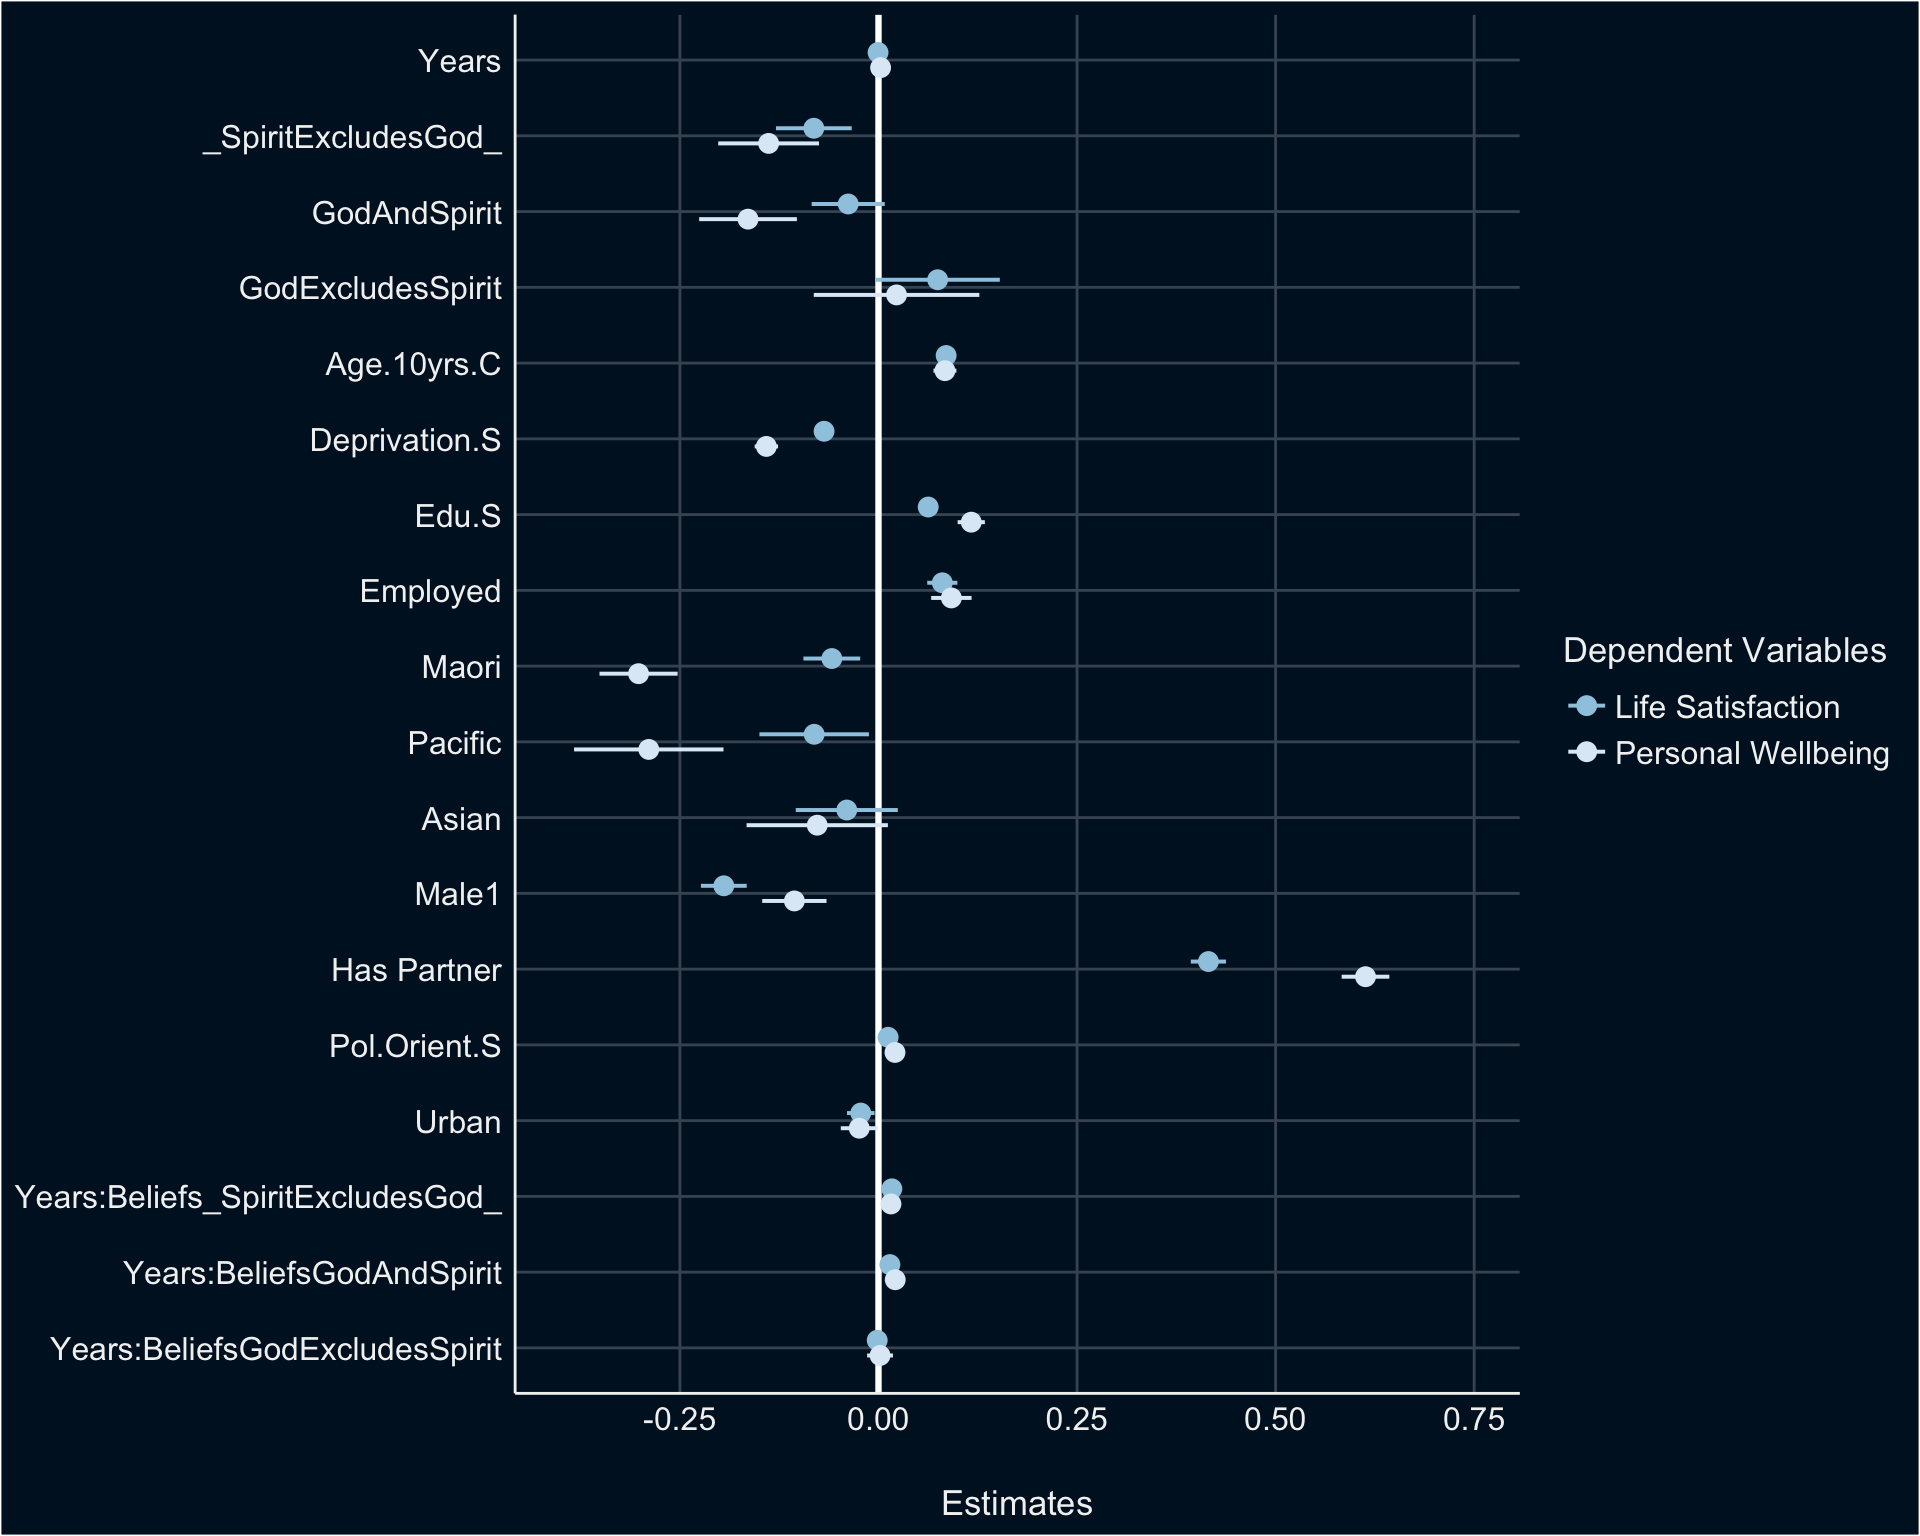
\includegraphics[width=6.4in]{Figs/USEcoefficientplots-1} \caption{Combination Coefficient Plots for Personal Well-being and Life Satisfaction Spirit Belief Longitudinal Models}\label{fig:unnamed-chunk-1}
\end{figure}

Table 2 about here:

\[
\begin{table}
\centering 
\caption{"Longitudinal Models"}\label{}
\scalebox{0.6}{
\begin{tabular}{l c c}
\toprule
 & Personal Well-Being & Life Satisfaction \\
\midrule
(Intercept)                        & $\mathbf{6.63}^{***}$  & $\mathbf{4.94}^{***}$  \\
                                   & $(0.03)$               & $(0.02)$               \\
Years                              & $0.00$                 & $-0.00$                \\
                                   & $(0.00)$               & $(0.00)$               \\
Beliefs\_SpiritExcludesGod\_       & $\mathbf{-0.14}^{***}$ & $\mathbf{-0.08}^{***}$ \\
                                   & $(0.03)$               & $(0.02)$               \\
BeliefsGodAndSpirit                & $\mathbf{-0.16}^{***}$ & $-0.04$                \\
                                   & $(0.03)$               & $(0.02)$               \\
BeliefsGodExcludesSpirit           & $0.02$                 & $0.07$                 \\
                                   & $(0.05)$               & $(0.04)$               \\
Age.10yrs.C                        & $\mathbf{0.08}^{***}$  & $\mathbf{0.09}^{***}$  \\
                                   & $(0.01)$               & $(0.01)$               \\
Deprivation.S                      & $\mathbf{-0.14}^{***}$ & $\mathbf{-0.07}^{***}$ \\
                                   & $(0.01)$               & $(0.01)$               \\
Edu.S                              & $\mathbf{0.12}^{***}$  & $\mathbf{0.06}^{***}$  \\
                                   & $(0.01)$               & $(0.01)$               \\
Employed1                          & $\mathbf{0.09}^{***}$  & $\mathbf{0.08}^{***}$  \\
                                   & $(0.01)$               & $(0.01)$               \\
EthnicCatsMaori                    & $\mathbf{-0.30}^{***}$ & $\mathbf{-0.06}^{**}$  \\
                                   & $(0.03)$               & $(0.02)$               \\
EthnicCatsPacific                  & $\mathbf{-0.29}^{***}$ & $\mathbf{-0.08}^{*}$   \\
                                   & $(0.05)$               & $(0.04)$               \\
EthnicCatsAsian                    & $-0.08$                & $-0.04$                \\
                                   & $(0.05)$               & $(0.03)$               \\
Male1                              & $\mathbf{-0.11}^{***}$ & $\mathbf{-0.19}^{***}$ \\
                                   & $(0.02)$               & $(0.01)$               \\
Partner1                           & $\mathbf{0.61}^{***}$  & $\mathbf{0.42}^{***}$  \\
                                   & $(0.02)$               & $(0.01)$               \\
Pol.Orient.S                       & $\mathbf{0.02}^{***}$  & $\mathbf{0.01}^{**}$   \\
                                   & $(0.01)$               & $(0.00)$               \\
UrbanUrban                         & $\mathbf{-0.02}^{*}$   & $\mathbf{-0.02}^{*}$   \\
                                   & $(0.01)$               & $(0.01)$               \\
Years:Beliefs\_SpiritExcludesGod\_ & $\mathbf{0.02}^{**}$   & $\mathbf{0.02}^{***}$  \\
                                   & $(0.00)$               & $(0.00)$               \\
Years:BeliefsGodAndSpirit          & $\mathbf{0.02}^{***}$  & $\mathbf{0.01}^{***}$  \\
                                   & $(0.00)$               & $(0.00)$               \\
Years:BeliefsGodExcludesSpirit     & $0.00$                 & $-0.00$                \\
                                   & $(0.01)$               & $(0.01)$               \\
\midrule
AIC                                & $248580.18$            & $200599.16$            \\
BIC                                & $248775.08$            & $200793.96$            \\
Log Likelihood                     & $-124269.09$           & $-100278.58$           \\
Num. obs.                          & $79270$                & $78888$                \\
Num. groups: Id                    & $20979$                & $20972$                \\
Var: Id (Intercept)                & $1.78$                 & $0.88$                 \\
Var: Residual                      & $0.74$                 & $0.42$                 \\
\bottomrule
\multicolumn{3}{l}{\scriptsize{$^{***}p<0.001$; $^{**}p<0.01$; $^{*}p<0.05$}}
\end{tabular}
}
\end{table}
\]

\hypertarget{personal-well-being}{%
\subsection{Personal Well-Being}\label{personal-well-being}}

We fitted a linear mixed model (estimated using REML and nloptwrap optimizer) to predict personal well-being (PWI) with Years (0-9), Beliefs (four categories), Age.10yrs.C, Deprivation.S, Edu.S, Employed, EthnicCats, Male, Partner, Pol.Orient.S and Urban, with Id as random effects. The model included Id as random effects. The model's intercept, corresponding to Years = 0, Beliefs = Skeptic, Age = (sample mean), Deprivation.S = (sample mean), Edu.S =(sample mean), Employed = Not Employed, EthnicCats = Euro, Male = Not Mail, Partner = No Partner, Pol.Orient.S = (sample mean),, Urban = Not Urban and Id = 2, is at 4.94 (SE = 0.02, 95\% CI {[}4.89, 4.99{]}, p \textless{} .001) is at 6.63 (SE = 0.03, 95\% CI {[}6.57, 6.70{]}, p \textless{} .001). Within this model:

\begin{itemize}
\tightlist
\item
  The effect of Years is positive is not reliable (beta = 2.66e-03, SE = 3.58e-03, std. beta = 3.19e-03, p = 0.458). We infer that Skeptics personal well-being is not increasing in the Skeptic population
\item
  The effect of Beliefs\_SpiritExcludesGod\_is reliably negative (beta = -0.14, SE = 0.03, std. beta = -0.03, p \textless{} .001). We infer that overall the population that believes in a Spirit but does not believe in a God is expected to have a lower personal well-being than skeptics.
\item
  The effect of BeliefsGodAndSpirit is reliably negative (beta = -0.16, SE = 0.03, std. beta = -0.02, p \textless{} .001). We infer that overall the population that believes in God and a spirit or life force is expected to have a lower Personal Well-being than skeptics.
\item
  The effect of BeliefsGodExcludesSpirit is not reliably different from the skeptic population (beta = 0.02, SE = 0.05, std. beta = 0.02, p = 0.669).
\item
  The effect of Age.10yrs.C is reliably positive (beta = 0.08, SE = 7.38e-03, std. beta = 0.07, p \textless{} .001). Older people have greater personal well-beingwellbeing.
\item
  The effect of Deprivation.S is reliably negative (beta = -0.14, SE = 7.50e-03, std. beta = -0.08, p \textless{} .001). Deprived people have lower personal well-beingwellbeing.
\item
  The effect of Edu.S is reliably positive (beta = 0.12, SE = 8.74e-03, std. beta = 0.07, p \textless{} .001). Educated people greater personal well-beingwellbeing
\item
  The effect of Employed is reliably positive (beta = 0.09, SE = 0.01, std. beta = 0.05, p \textless{} .001). Employed people have greater personal well-beingwellbeing.
\item
  The effect of EthnicCatsMaori is reliably negative (beta = -0.30, SE = 0.03, std. beta = -0.18, p \textless{} .001).
\item
  The effect of EthnicCatsPacific is reliably negative (beta = -0.29, SE = 0.05, std. beta = -0.17, p \textless{} .001).
\item
  The effect of EthnicCatsAsian is not reliable (beta = -0.08, SE = 0.05, std. beta = -0.05, p = 0.089).
\item
  The effect of Male is reliably negative (beta = -0.11, SE = 0.02, std. beta = -0.06, p \textless{} .001).
\item
  The effect of Having a Partner is reliably positive (beta = 0.61, SE = 0.02, std. beta = 0.37, p \textless{} .001).
\item
  The effect of Pol.Orient.S is reliably positive (beta = 0.02, SE = 5.67e-03, std. beta = 0.01, p \textless{} .001).
\item
  The effect of Urban is reliably negative (beta = -0.02, SE = 0.01, std. beta = -0.01, p \textless{} .05).
\end{itemize}

\hypertarget{personal-well-being-years-x-beliefs}{%
\subsection{Personal well-being: years X beliefs}\label{personal-well-being-years-x-beliefs}}

\begin{figure}
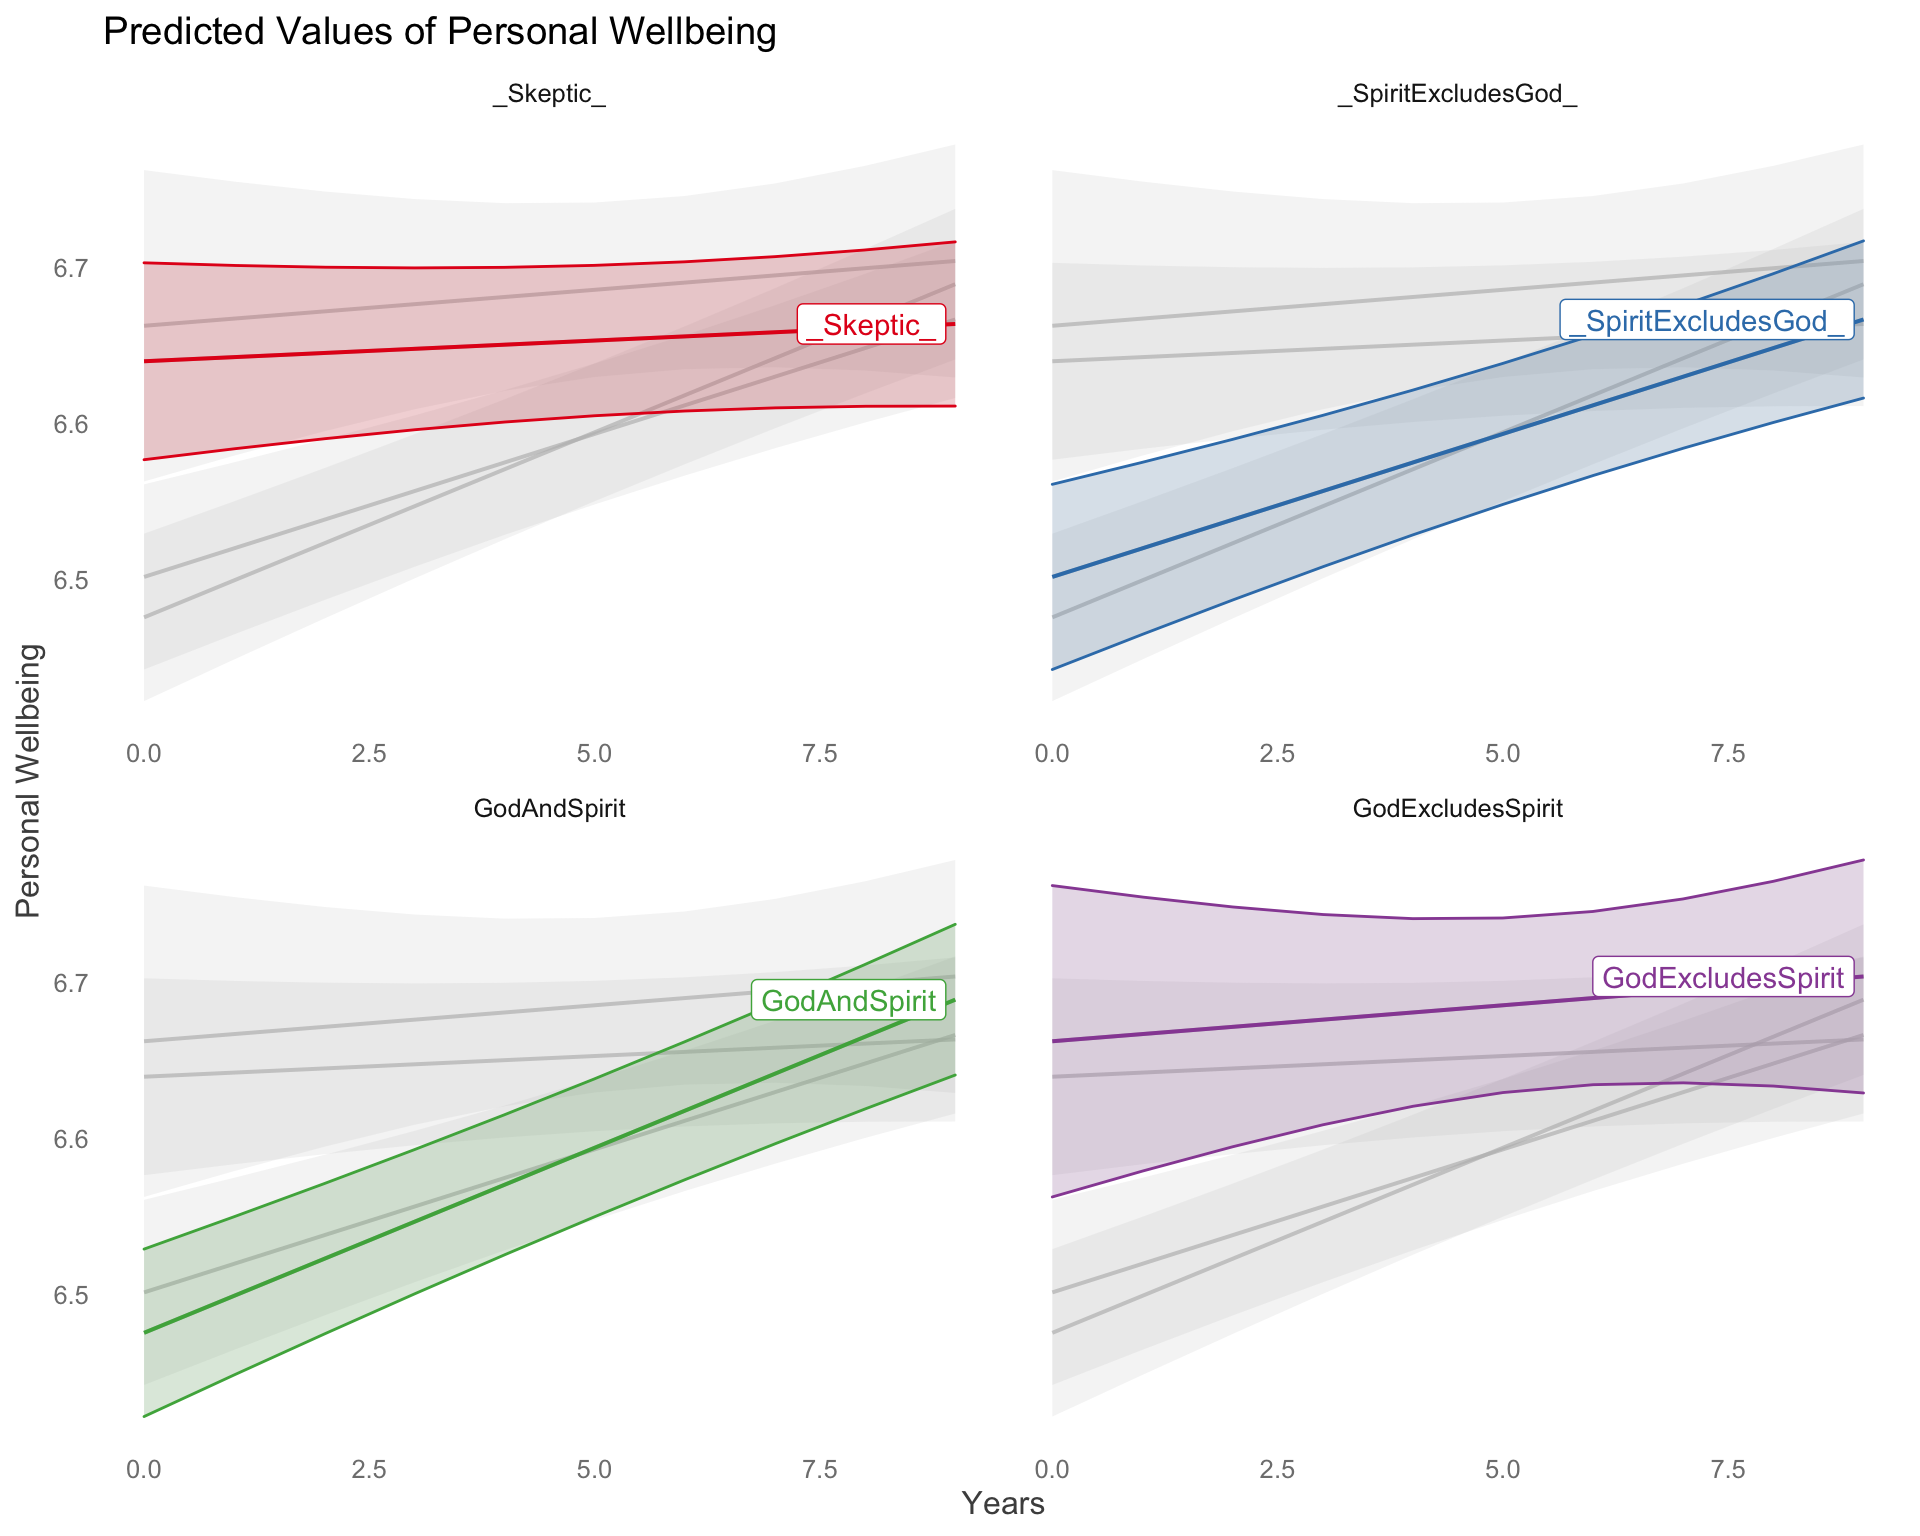
\includegraphics[width=6.4in]{Figs/USEPWI_expected-1} \caption{Combination Coefficient Plots for Personal Well-being and Life Satisfaction Spirit Belief Longitudinal Models}\label{fig:unnamed-chunk-2}
\end{figure}

Focusing on the interaction of time with belief-type on personal well-being we observe:

\begin{itemize}
\tightlist
\item
  The effect of Years X SpiritExcludesGod\_ is reliably positive (beta = 0.02, SE = 4.86e-03, std. beta = 0.02, p \textless{} .01). We infer that, unlike the skeptic population, people with beliefs in a spirit or life force who do not believe in a God tend to grow in their personal well-being over time.
\item
  The effect of Years X GodAndSpirit is reliably positive (beta = 0.02, SE = 4.41e-03, std. beta = 0.03, p \textless{} .001). We infer that people who believe in a spirit or life force who also believe in a God tend to grow in their personal well-being over time
\item
  The effect of Years X GodExcludesSpirit is not reliable(beta = 1.96e-03, SE = 8.29e-03, std. beta = 2.36e-03, p = 0.813). Thus, God believers who doubt in a Spirit or Life Force start maintain higher personal well-being than do other groups, but they are not expected to grow in personal well-being over time.
\end{itemize}

\hypertarget{life-satisfaction}{%
\subsection{Life Satisfaction}\label{life-satisfaction}}

We fitted a linear mixed model (estimated using REML and nloptwrap optimizer) to predict Life Satisfaction (LIFESAT) with Years (0-9), Beliefs (four categories), Age.10yrs.C, Deprivation.S, Edu.S, Employed, EthnicCats, Male, Partner, Pol.Orient.S and Urban, with Id as random effects. Standardized parameters were obtained by fitting the model on a standardized version of the dataset.The model's total explanatory power is substantial (conditional R2 = 0.69). The model's intercept, corresponding to Years = 0, Beliefs = Skeptic, Age = (sample mean),, Deprivation.S = (sample mean), Edu.S =(sample mean), Employed = Not Employed, EthnicCats = Euro, Male = Not Mail, Partner = No Partner, Pol.Orient.S = (sample mean), Urban = Not Urban and Id = 2, is at 4.94 (SE = 0.02, 95\% CI {[}4.89, 4.99{]}, p \textless{} .001). Within this model:

\begin{itemize}
\tightlist
\item
  The effect of Years is not reliable (beta = -5.50e-04, SE = 2.69e-03, std. beta = -9.32e-04, p = 0.838). We do not infer growth over time in Life Satisfaction among the Skeptic population
\item
  The effect of BeliefsSpiritExcludesGod is reliably negative (beta = -0.08, SE = 0.02, std. beta = 0.01, p \textless{} .001). We infer that overall the population that believes in a Spirit but does not believe in a God is expected to have a lower Life Satisfaction than skeptics.
\item
  The effect of BeliefsGodAndSpirit is not reliable (beta = -0.04, SE = 0.02, std. beta = 0.04, p = 0.105). We do not infer growth over time in Life Satisfaction among this (Skeptic) population
\item
  The effect of BeliefsGodExcludesSpirit is reliably positive (beta = 0.07, SE = 0.04, std. beta = 0.05, p = 0.062).We infer that overall the population that believes in a God but does not believe in a spirit is not reliably different from the Skeptics population in Life Satisfaction.
\item
  The effect of Age.10yrs.C is reliably positive (beta = 0.09, SE = 5.26e-03, std. beta = 0.10, p \textless{} .001). Older people have greater Life Satisfaction
\item
  The effect of Deprivation.S is is reliably negative (beta = -0.07, SE = 5.50e-03, std. beta = -0.06, p \textless{} .001). People who are more deprived have lower Life Satisfaction.
\item
  The effect of Edu.S is reliably positive (beta = 0.06, SE = 6.33e-03, std. beta = 0.05, p \textless{} .001). Educated people have greater Life Satisfaction
\item
  The effect of Employed is reliably positive (beta = 0.08, SE = 9.69e-03, std. beta = 0.07, p \textless{} .001). People who are employed tend to have greater Life Satisfaction
\item
  The effect of EthnicCatsMaori is reliably negative (beta = -0.06, SE = 0.02, std. beta = -0.05, p \textless{} .01). People who belong to the minority Maori group tend to have lower Life Satisfaction.
\item
  The effect of EthnicCatsPacific is reliably negative (beta = -0.08, SE = 0.04, std. beta = -0.07, p \textless{} .05). People who belong to the minority Pacific peoples group tend to have lower life satisfaction.
\item
  The effect of EthnicCatsAsian is not reliably different from people of European ethnicity in life satisfaction(beta = -0.04, SE = 0.03, std. beta = -0.03, p = 0.223).
\item
  The effect of Male is reliably negative (beta = -0.19, SE = 0.01, std. beta = -0.16, p \textless{} .001).
\item
  The effect of HasPartner is reliably positive (beta = 0.42, SE = 0.01, std. beta = 0.35, p \textless{} .001).
\item
  The effect of Pol.Orient.S is reliably positive (beta = 0.01, SE = 4.23e-03, std. beta = 0.01, p \textless{} .01).
\item
  The effect of Urban is reliably negative (beta = -0.02, SE = 8.85e-03, std. beta = -0.02, p \textless{} .05).
\end{itemize}

\hypertarget{life-satisfaction-years-x-beliefs}{%
\subsection{Life Satisfaction: years X beliefs}\label{life-satisfaction-years-x-beliefs}}

\begin{figure}
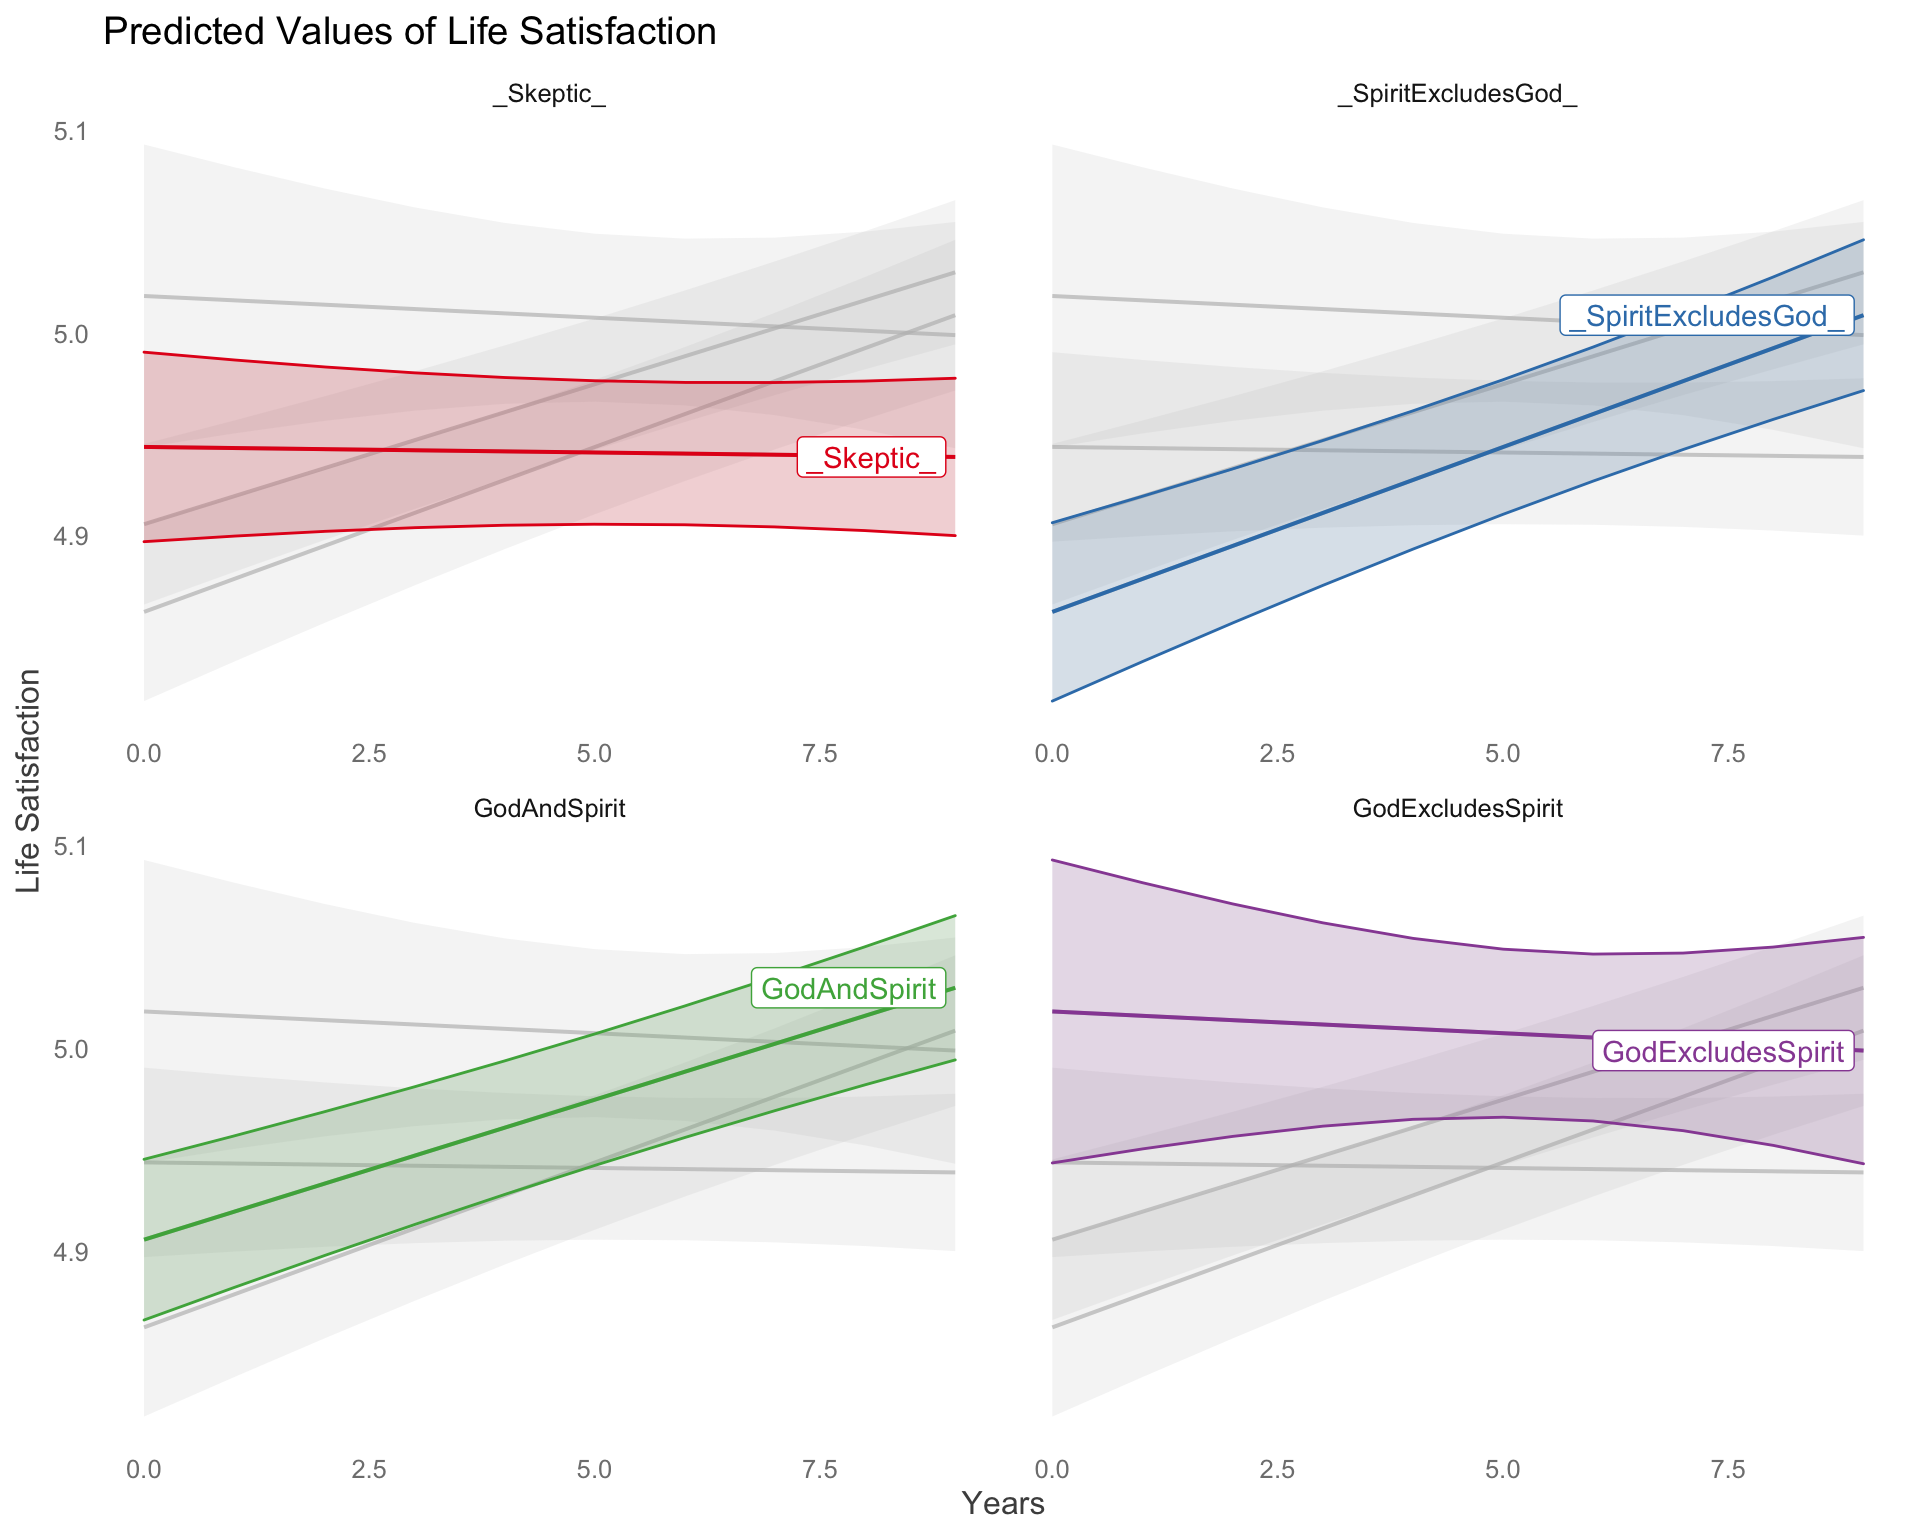
\includegraphics[width=6.4in]{Figs/USElifsat_expected-1} \caption{Prediction Plot Life Satisfaction Spirit Belief Longitudinal Models}\label{fig:unnamed-chunk-3}
\end{figure}

\begin{itemize}
\tightlist
\item
  The interaction of Years X Beliefs\_SpiritExcludesGod\_ is reliably positive (beta = 0.02, SE = 3.66e-03, std. beta = 0.03, p \textless{} .001). We infer that, unlike the Skeptic population, people with beliefs in a Spirit or Life Force who do not believe in a God tend to grow in their Life Satisfaction over time.

  \begin{itemize}
  \tightlist
  \item
    The interaction of Years X BeliefsGodAndSpirit is reliably positive (beta = 0.01, SE = 3.32e-03, std. beta = 0.02, p \textless{} .001). We infer that people who believe in a spirit or life force who also believe in a God tend to grow in their Life Satisfaction over time
  \item
    The effect of Years X BeliefsGodExcludesSpirit is not reliable (beta = -1.59e-03, SE = 6.25e-03, std. beta = -2.70e-03, p = 0.799). Thus, God believers who doubt in a Spirit or Life Force start maintain higher Life-Satisfaction than do other groups, but they are not expected to grow in Life-Satisfaction over time.
  \end{itemize}
\end{itemize}

\hypertarget{imputed-data-analysis}{%
\subsection{Imputed data analysis}\label{imputed-data-analysis}}

To adjust for potential biases from missing responses, we conducted a supplementary analysis in which we imputed missing values over the the longitudinal sample. This analysis is describe in Supplement 1. Averaging over the missing responses does not change inference, however we observe growth across all four groups in both personal well-being and life satisfaction. Additionally we observe substantially stronger effects for the slope of Spirit Beliefs on both personal well-being and life-satisfaction. Figures 3 and Figures 4 describe the predicted slopes of change. The inference from this analysis remains the same as from the analysis in which we delete missing values row-wise, by panel wave. In all analyses those who believe in a spirit or life-force are expected to experience greater growth in well-being over time.

Figure 3 about here

\begin{figure}
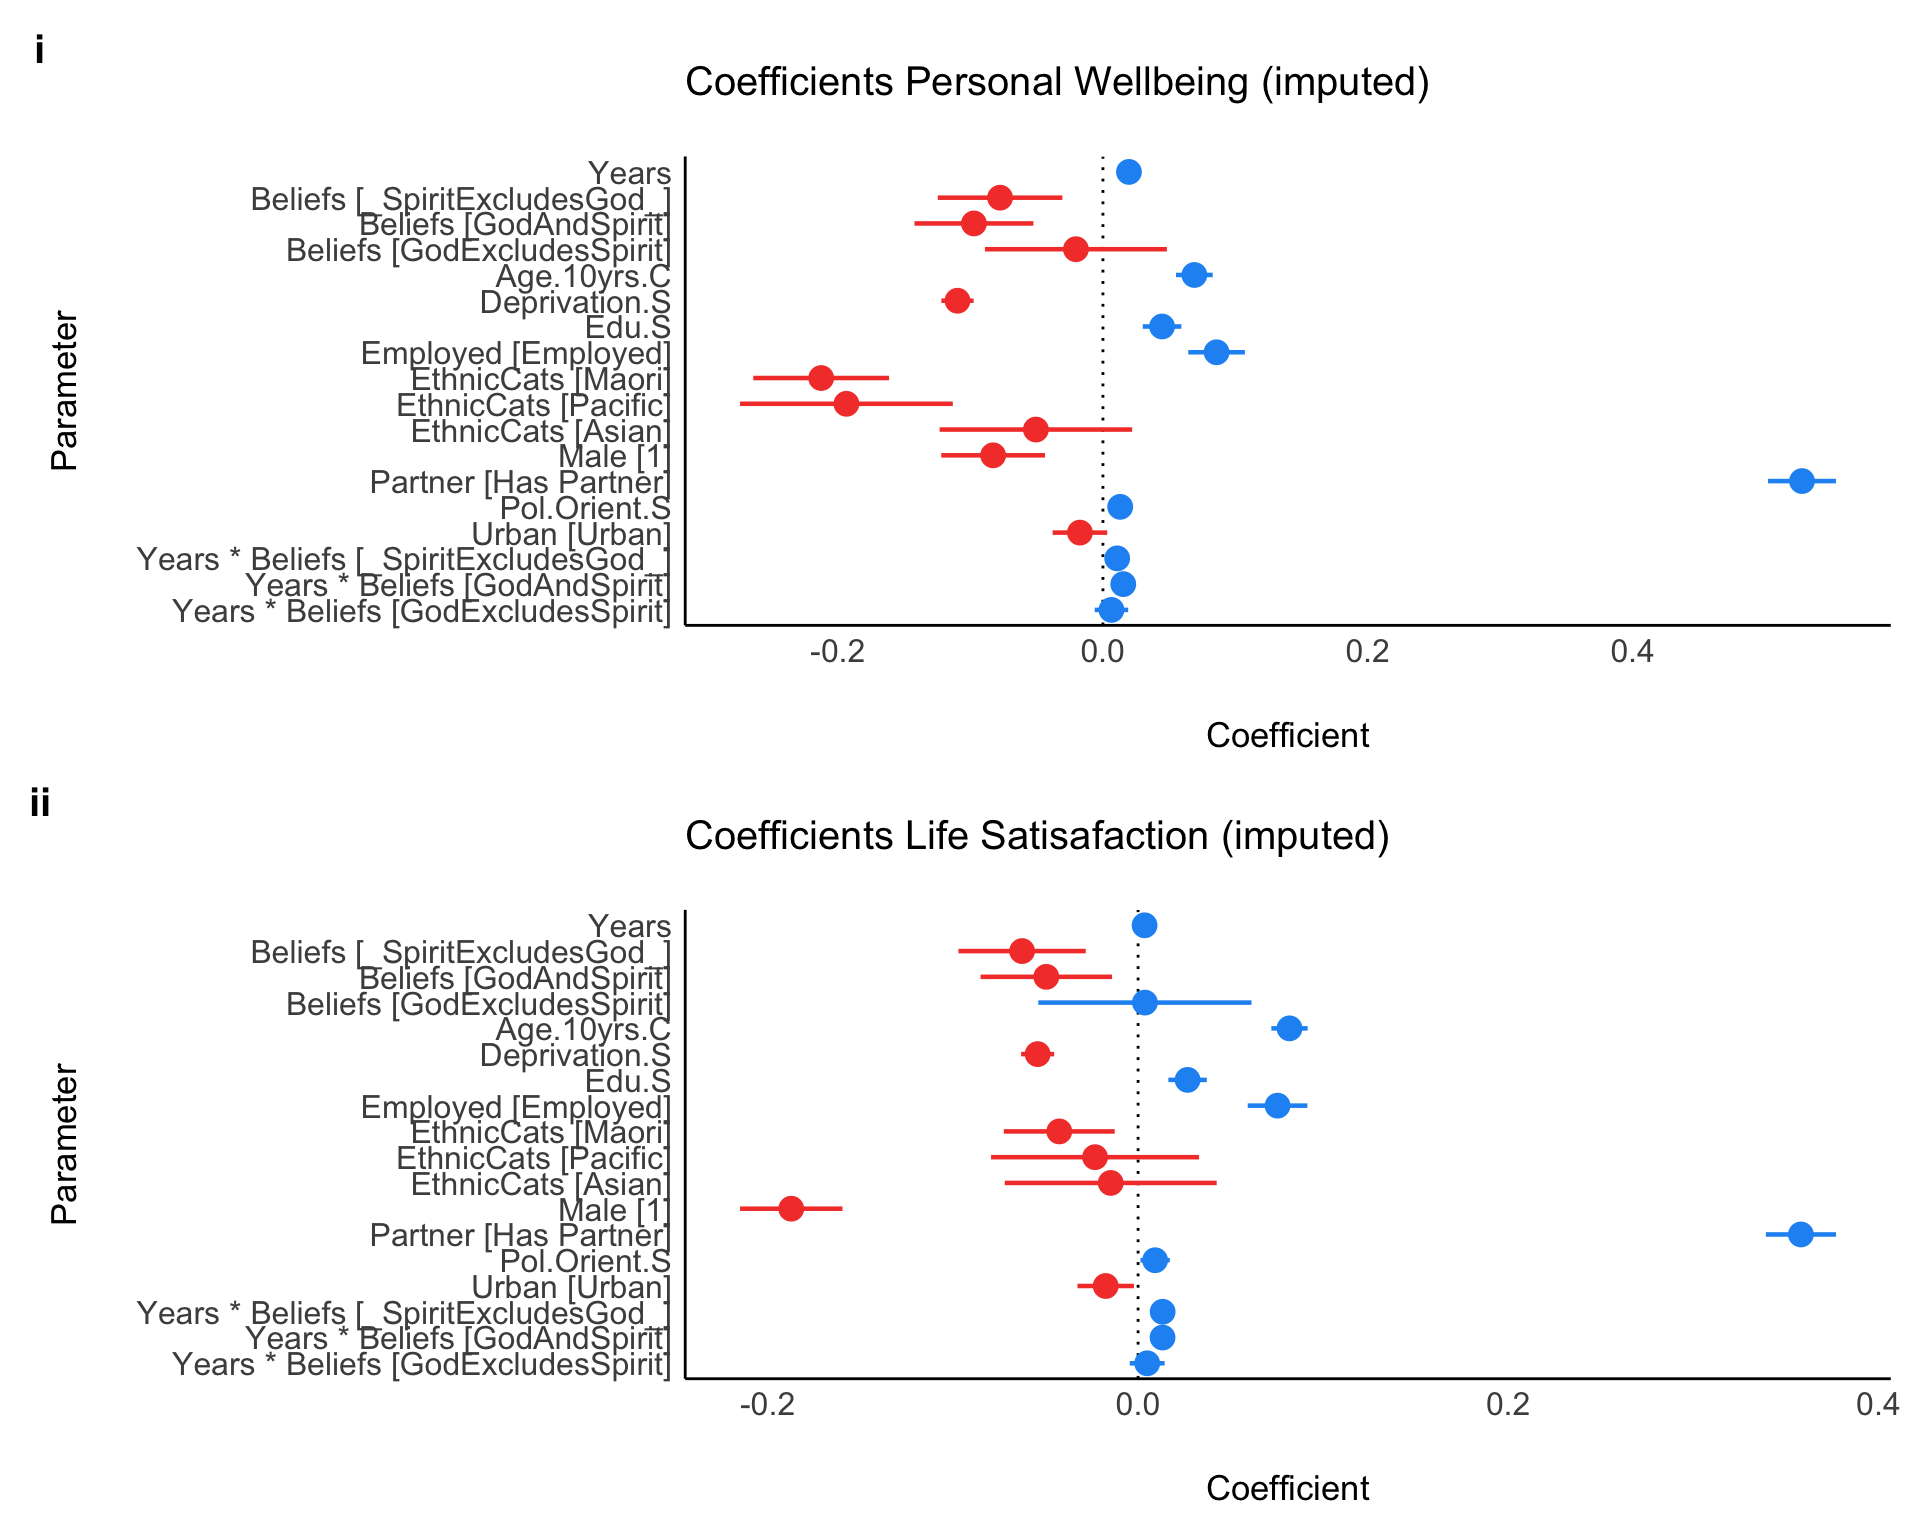
\includegraphics[width=6.4in]{Figs/coefficient_plot_both_imputed-1} \caption{Imputed data analysis: coefficient plot}\label{fig:unnamed-chunk-4}
\end{figure}

Figure 4 about here

\begin{figure}
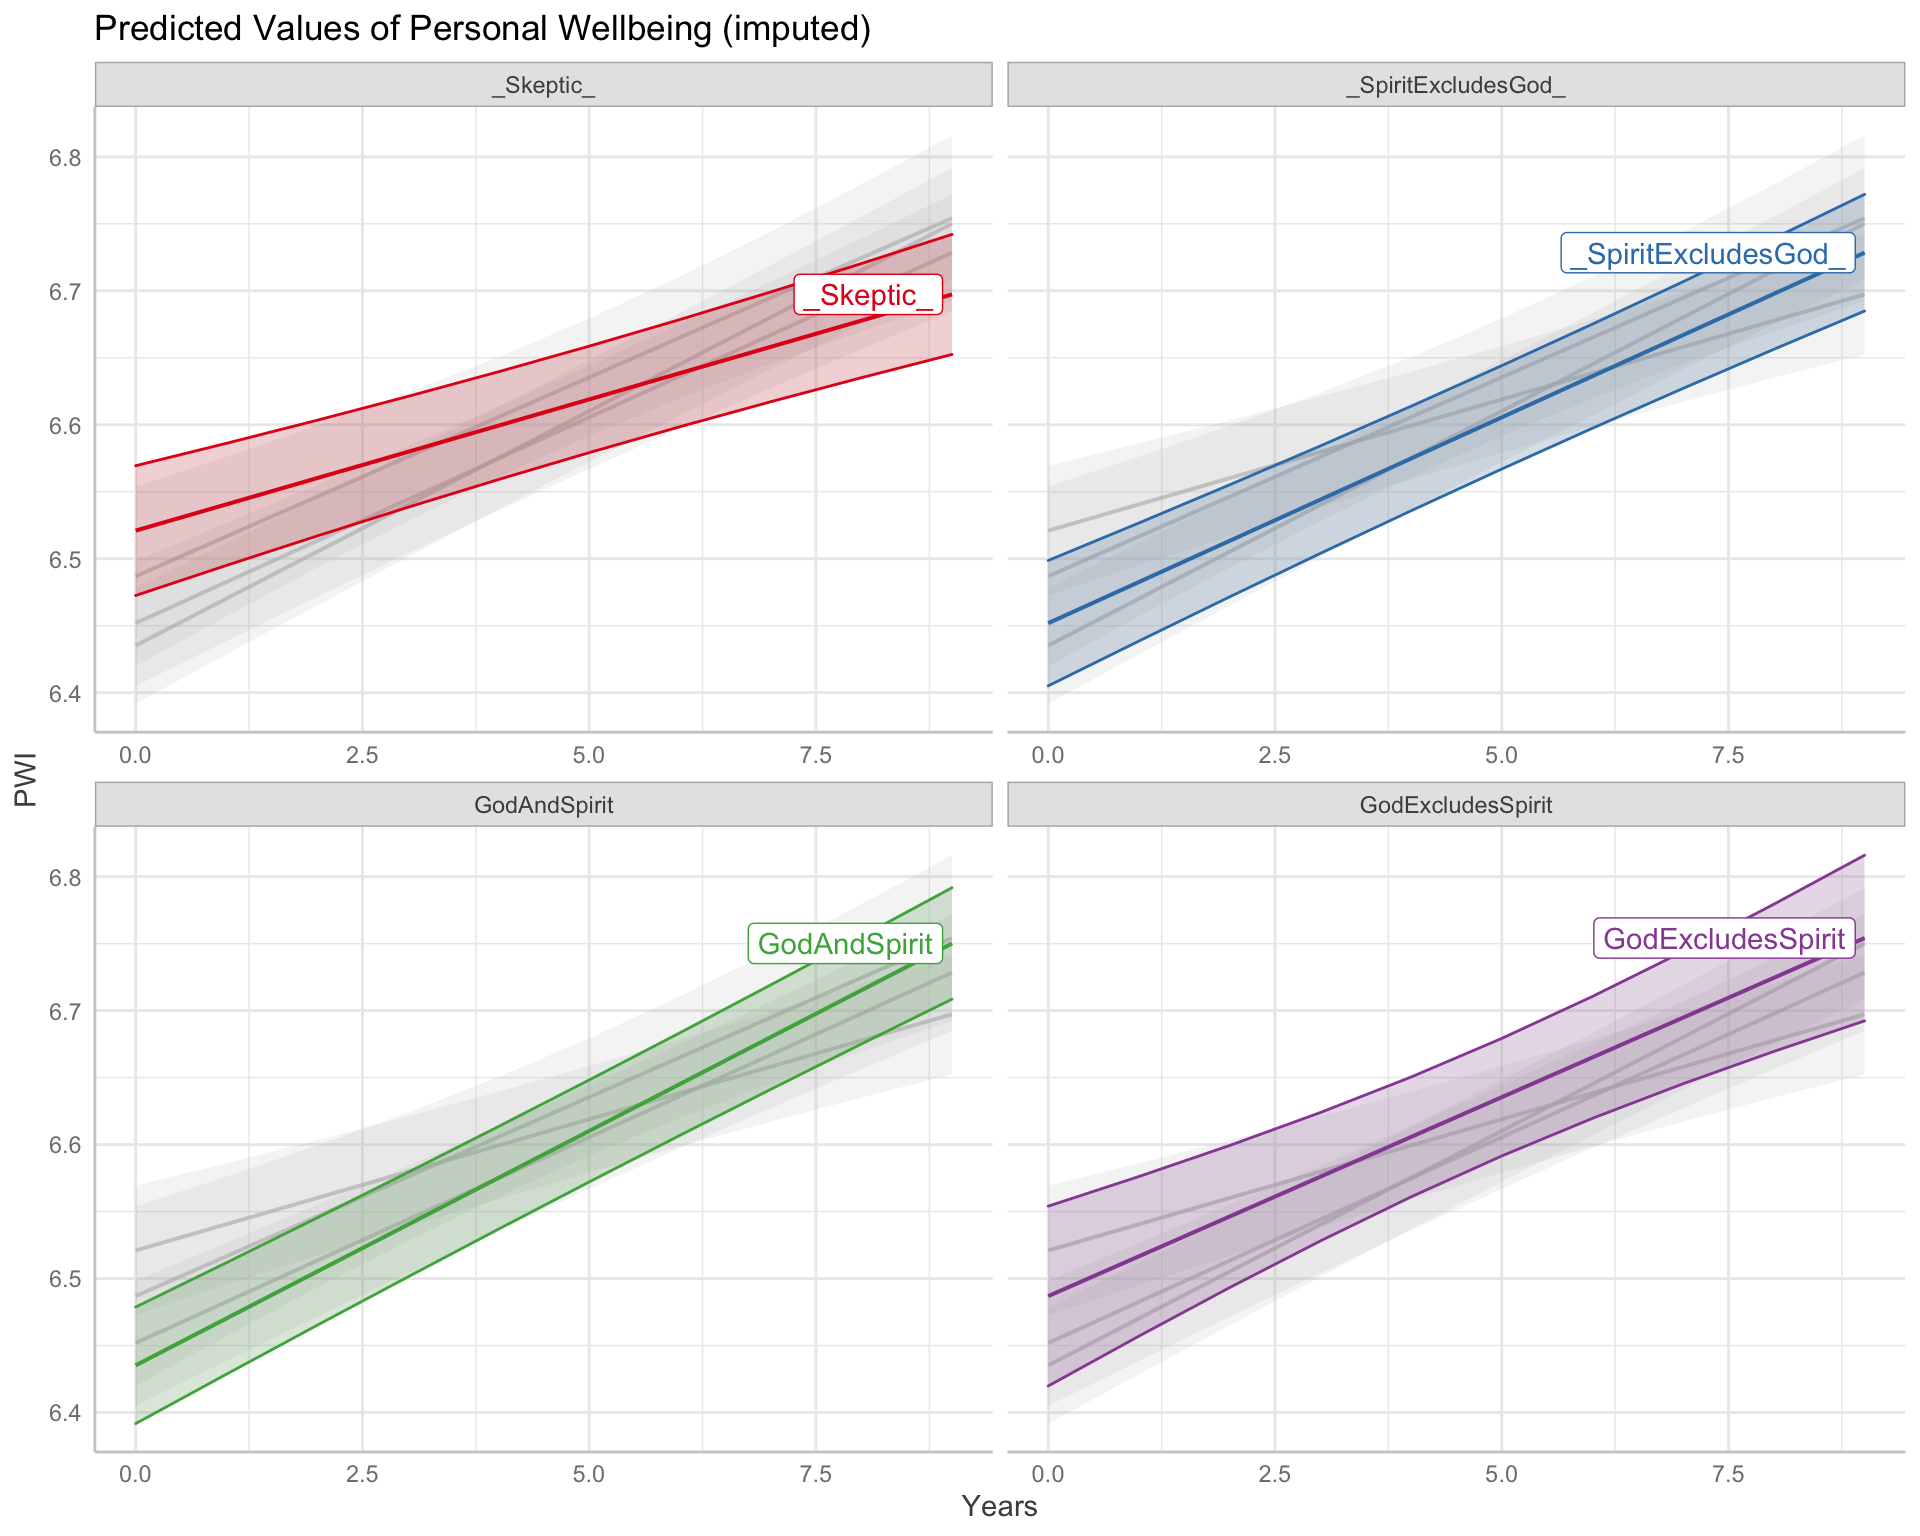
\includegraphics[width=6.4in]{Figs/predicted_PWI_impute-1} \caption{Imputed data analysis: predicted personal wellbeing by years X beliefs}\label{fig:unnamed-chunk-5}
\end{figure}

Figure 5 about here

\begin{figure}
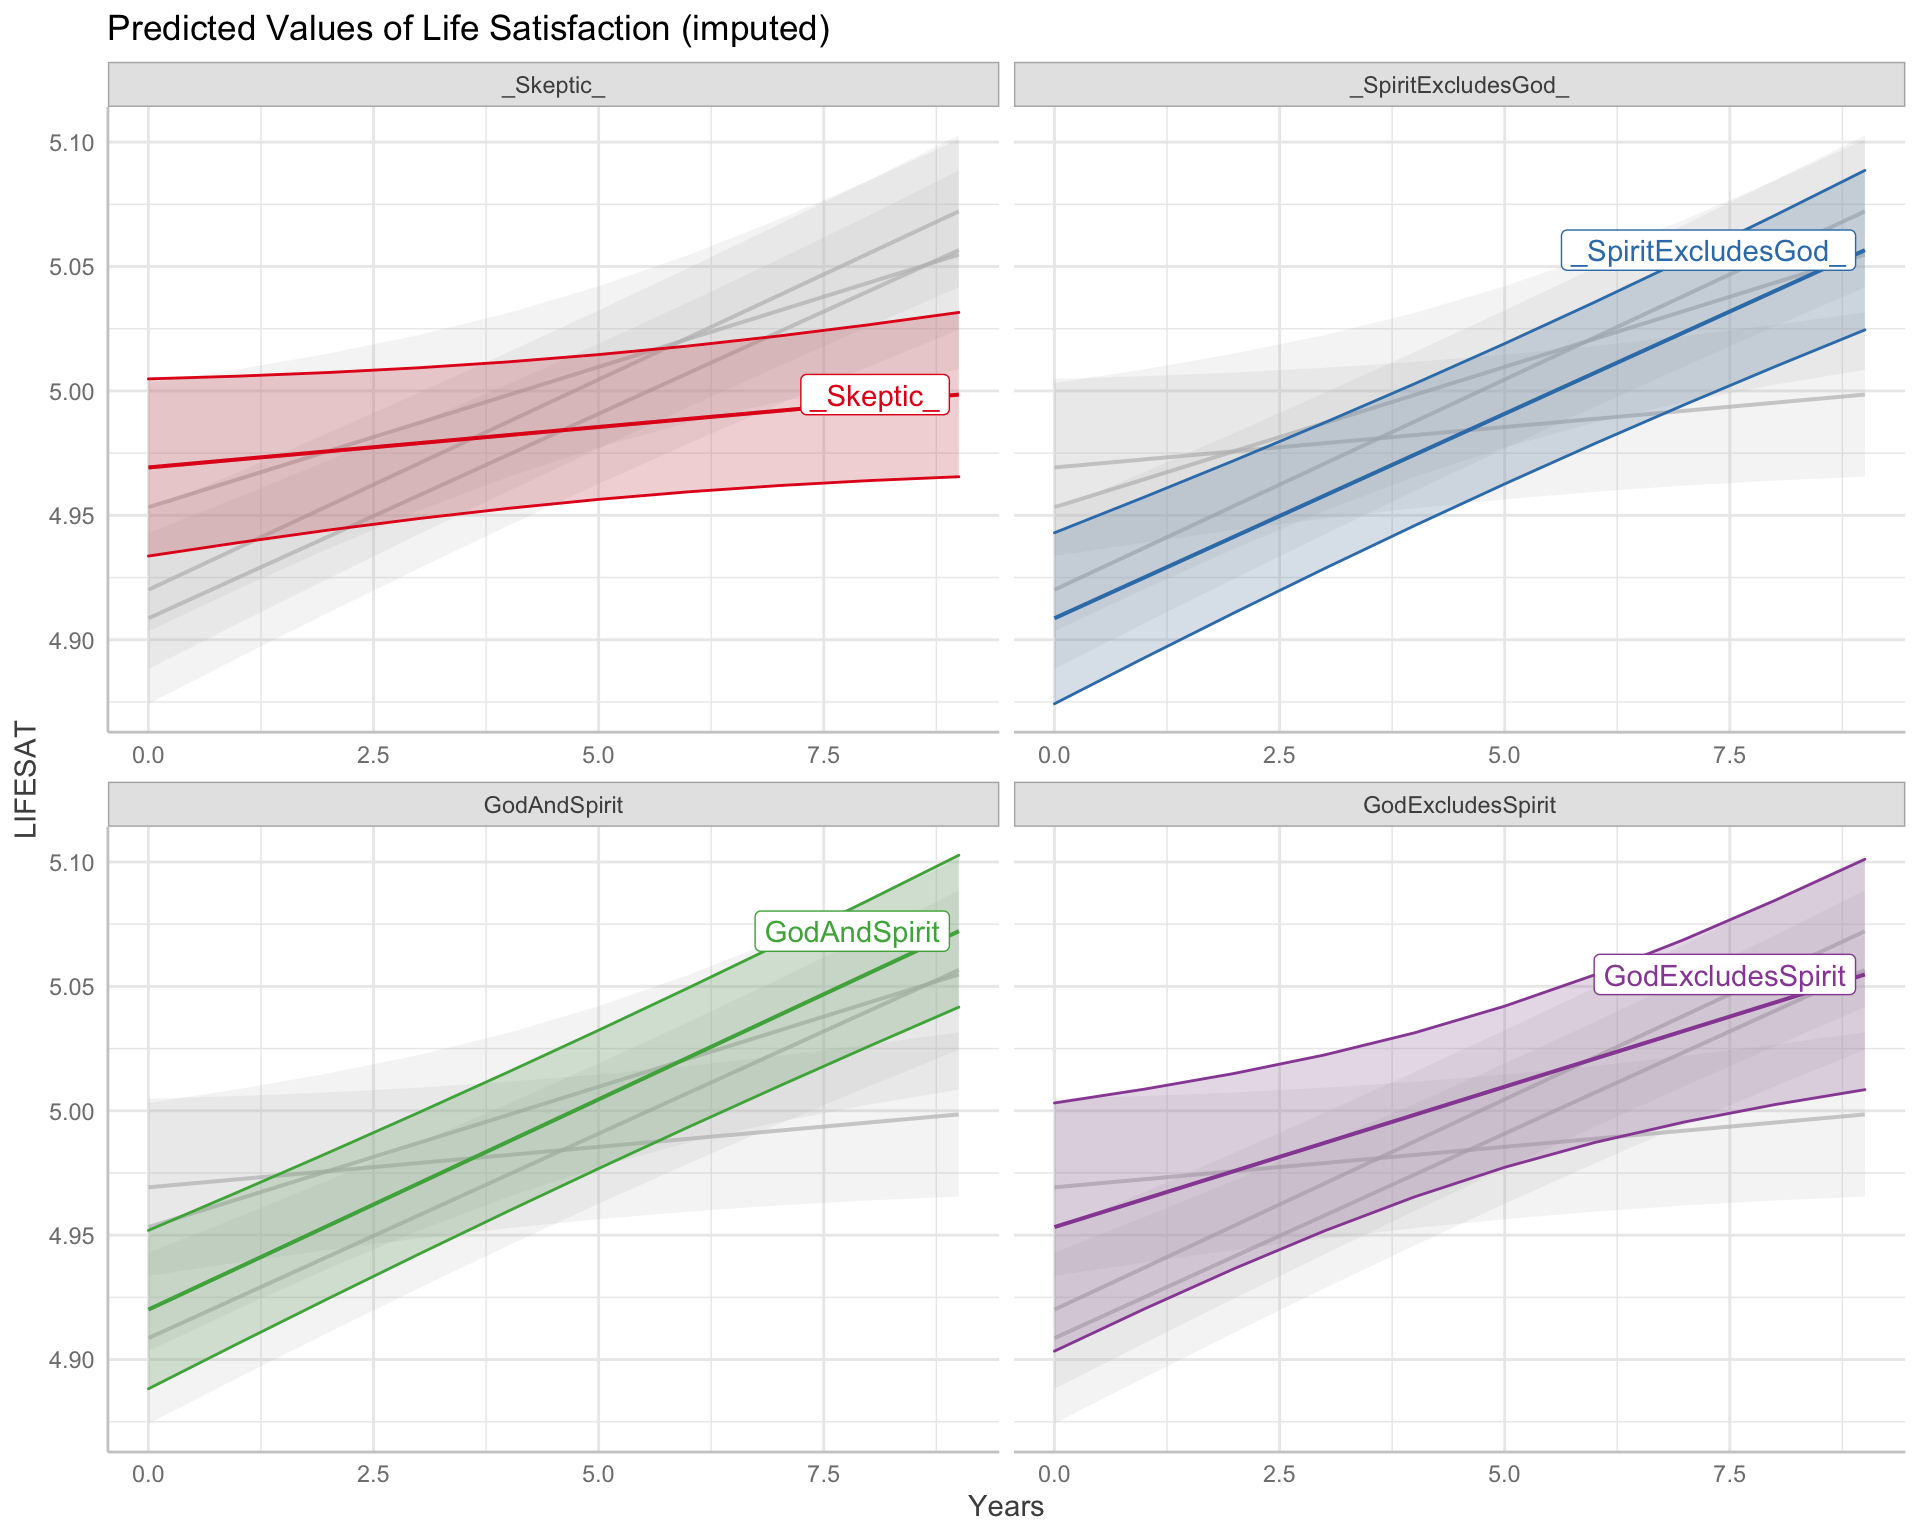
\includegraphics[width=6.4in]{Figs/predicted_lifesat_imputed-1} \caption{Imputed data analysis: predicted personal wellbeing by years X beliefs}\label{fig:unnamed-chunk-6}
\end{figure}

\hypertarget{discussion}{%
\section{Discussion}\label{discussion}}

The purpose of this study has been to clarify the relationship between belief in a spirit/life force and subjective well-being, addressing three challenges from previous research: (1) tautological measures of spirituality and subjective well-being; (2) insufficiently distinct measures of spirituality and religion; (3) cross-sectional samples. Here, we ask whether beliefs in a Spirit or Life Force predict growth in personal well-being and life-satisfaction over eight years in populations who differ in the this belief, and who also differ in their belief in a God. We find that

These findings demonstrate the importance of investigating spiritual beliefs as a domain of interest in its own right. In many Western countries, people are increasingly identifying as \enquote{spiritual but not religious} (Swinton, 2001; Zinnbauer \& Pargament, 2005). Other studies find that those who have a spiritual understanding of life without a religious framework are at an increased risk of having mental disorders (King et al., 2013). As such, it is important to understand the ramifications of belief in a spirit for psychological health.
To assess the relationship between a belief in a spirit or life force and subjective well-being, we improve upon past methods in three ways.

Despite the opposition of our findings to those of many previous studies, there is room for agreement. We show that over time both \enquote{BXG} and \enquote{BIG} are associated with marginally better subjective well-being. As seen in Figure 2., both \enquote{BXG} and \enquote{BIG} predict marginally higher personal well-being and life satisfaction as time progresses. So, while those who adhere to these beliefs may start out below their skeptic counterparts in terms of their subjective well-being, they do eventually catch up. We also find that their life satisfaction is actually improving at a greater rate than skeptics. Thus, in the long term, both sustained \enquote{BXG} and \enquote{BIG} may actually be associated with better subjective well-being.

Our results also help to clarify the relationship among religion, spirituality, and subjective well-being outcomes. BXG and BIG performed almost identically in terms of their ability to predict subjective well-being outcomes. This trend suggests that any kind of existential belief - regardless of whether a god is involved - might affect subjective well-being in much the same way. This result is good news as increasing numbers of individuals continue to report spiritual but not necessarily religious beliefs.

Taken as a whole, our results cannot refute the entire narrative of the positive relationship between spirituality and emotional well-being. First, our analysis focuses only on belief. While belief is an important part of spirituality it is not by any means spirituality itself. Individuals may identify as spiritual without any accompanying belief in a spirit or life force. Moreover, practices and rituals associated with different forms of spirituality that were not tested in this study may have large effects. Second, despite flawed methods, past studies may still be accurate. New Zealand is a largely secular country, so belief in a spirit or life force may have different impacts on subjective well-being outcomes in this context than in other, more religious contexts. Overall, though, our findings add to the existing literature, helping to untangle the multifaceted relationship among religion, spirituality, and subjective well-being.

\hypertarget{limitations}{%
\subsection{Limitations}\label{limitations}}

This article makes useful contributions to the continued debate regarding the relationship between religion and spirituality and mental health outcomes, but it is important to acknowledge several limitations. First, we relied upon self-reported data from the NZAVS. Although this is an accurate method for measuring belief in a spirit or life force, it may be a less accurate manner of measuring subjective well-being. It is possible that self-administration of our emotional well-being (personal well-being and life satisfaction) scales could result in mismeasurement. Second, we may not capture the full range spiritualities, which likely extend beyond belief and might even be inherently emotional. Thus, while our method avoided tautology, it might have also excluded participants who consider themselves to be spiritual but do not subscribe to a belief in a spirit or life force.

\hypertarget{authors-contributions}{%
\subsubsection{Authors contributions}\label{authors-contributions}}

CS leads and manages the NZAVS, and collected the data for this study. BH and JB conceived
of the study. BH wrote the first draft of the manuscript and performed the analysis with input from JB. BH conducted background research and scientific literature review. All authors contributed substantially to the intellectual content of the study and the final manuscript.

\hypertarget{funding-statement}{%
\subsubsection{Funding statement}\label{funding-statement}}

The New Zealand Attitudes and Values Study is supported by a grant from the Templeton
Religion Trust (TRT0196). The funders had no role in the preparation of the article or the
decision to publish.

\hypertarget{supplemental-material}{%
\section{Supplemental Material}\label{supplemental-material}}

S1. Statistical Analysis in R
Statistical analysis was performed using R version 3.6.1 (2019-07-05). Platform: x86\_64-w64-mingw32 (64-bit), running under: Windows 10 (Action of the Toes). Generalized Linear Mixed Models were generated using the glmmTMB (Brooks et al.~2017; Knowles and Frederick 2019) package in R. In addition, we used the following R packages: dplyr (Hadley Wickham et al.~2019), tidyr (H. Wickham and Henry 2019), sjPlot (D. Lüdecke 2020), ggeffects (Daniel Lüdecke 2018), table1 and their dependencies.
Tables and coefficient plots were generated using the glmmTMB, ggeffects, and sjPlot packages in R. Models for both subjective well-being variables used family = gaussian, assuming a normal distribution. We ran each individual's unique ID as a random-effect. The tab\_model and plot\_model commands in sjPlot allowed for the creation of tables and coefficient plots. Predicted probability plots were generated using the ggpredict command in the ggeffects package. The table1 package in R was used for the creation of descriptive statistics tables.

\newpage

\hypertarget{references}{%
\section{References}\label{references}}

\begingroup
\setlength{\parindent}{-0.5in}
\setlength{\leftskip}{0.5in}

\hypertarget{refs}{}
\leavevmode\hypertarget{ref-Ano2005-hx}{}%
Ano, G. G., \& Vasconcelles, E. B. (2005). Religious coping and psychological adjustment to stress: A meta‐analysis. \emph{J. Clin. Psychol.}

\leavevmode\hypertarget{ref-Atkinson2014-ex}{}%
Atkinson, J., Salmond, C., \& Crampton, P. (2014). NZDep2013 index of deprivation. \emph{Wellington: Department of Public Health, University of Otago}.

\leavevmode\hypertarget{ref-Blackwell2017-oq}{}%
Blackwell, M., Honaker, J., \& King, G. (2017). A unified approach to measurement error and missing data: Details and extensions. \emph{Sociological Methods \& Research}.

\leavevmode\hypertarget{ref-Cummins2017-ur}{}%
Cummins, R. A., Eckerseley, R., Pallant, J., Van Vugt, J., \& Misajon, R. (2017). Australian unity wellbeing index. \emph{PsycTESTS Dataset}.

\leavevmode\hypertarget{ref-Diener1985-xy}{}%
Diener, E., Emmons, R. A., Larsen, R. J., \& Griffin, S. (1985). The satisfaction with life scale. \emph{Journal of Personality Assessment}.

\leavevmode\hypertarget{ref-Ellsworth2010-yu}{}%
Ellsworth, R. B., \& Ellsworth, J. B. (2010). Churches that enhance spirituality and wellbeing. \emph{Int. J. Appl. Psychoanal. Studies}, \emph{6}.

\leavevmode\hypertarget{ref-Garssen2016-km}{}%
Garssen, B., \& Visser, A. (2016). The association between religion/spirituality and mental health in cancer. \emph{Cancer}, \emph{122}(15), 2440.

\leavevmode\hypertarget{ref-Garssen2016-kb}{}%
Garssen, B., Visser, A., \& Jager Meezenbroek, E. de. (2016). Examining whether spirituality predicts subjective well-being: How to avoid tautology. \emph{Psycholog. Relig. Spiritual.}, \emph{8}(2), 141.

\leavevmode\hypertarget{ref-Ginsburg1995-jr}{}%
Ginsburg, M. L., Quirt, C., Ginsburg, A. D., \& MacKillop, W. J. (1995). Psychiatric illness and psychosocial concerns of patients with newly diagnosed lung cancer. \emph{CMAJ}, \emph{152}(5), 701--708.

\leavevmode\hypertarget{ref-Hackney2003-rs}{}%
Hackney, C. H., \& Sanders, G. S. (2003). Religiosity and mental health: A meta--analysis of recent studies. \emph{J. Sci. Study Relig.}

\leavevmode\hypertarget{ref-Honaker2011-yu}{}%
Honaker, J., King, G., Blackwell, M., \& Others. (2011). Amelia II: A program for missing data. \emph{J. Stat. Softw.}, \emph{45}(7), 1--47.

\leavevmode\hypertarget{ref-King2013-cg}{}%
King, M., Marston, L., McManus, S., Brugha, T., Meltzer, H., \& Bebbington, P. (2013). Religion, spirituality and mental health: Results from a national study of english households. \emph{British Journal of Psychiatry}.

\leavevmode\hypertarget{ref-Koenig2008-lv}{}%
Koenig, H. G. (2008). Concerns about measuring ``spirituality'' in research. \emph{J. Nerv. Ment. Dis.}, \emph{196}(5), 349.

\leavevmode\hypertarget{ref-Koenig2010-gk}{}%
Koenig, H. G. (2010). Spirituality and mental health. \emph{Int. J. Appl. Psychoanal. Studies}, \emph{15}.

\leavevmode\hypertarget{ref-Koenig2001-ow}{}%
Koenig, H. G., Associate Professor of Psychology and Religious Studies Michael E McCullough, PhD, McCullough, M. E., Larson, D. B., \& Adjunct Professor of Psychiatry David B Larson. (2001). \emph{Handbook of religion and health}. Oxford University Press.

\leavevmode\hypertarget{ref-Russinova2002-rq}{}%
Russinova, Z., Wewiorski, N. J., \& Cash, D. (2002). Use of alternative health care practices by persons with serious mental illness: Perceived benefits. \emph{Am. J. Public Health}, \emph{92}(10), 1600--1603.

\leavevmode\hypertarget{ref-Sawatzky2005-rw}{}%
Sawatzky, R., Ratner, P. A., \& Chiu, L. (2005). A Meta-Analysis of the relationship between spirituality and quality of life. \emph{Soc. Indic. Res.}, \emph{72}(2), 153--188.

\leavevmode\hypertarget{ref-Smith2003-re}{}%
Smith, T. B., McCullough, M. E., \& Poll, J. (2003). Religiousness and depression: Evidence for a main effect and the moderating influence of stressful life events. \emph{Psychol. Bull.}, \emph{129}(4), 614--636.

\leavevmode\hypertarget{ref-Swinton2001-vr}{}%
Swinton, J. (2001). \emph{Spirituality and mental health care: Rediscovering a 'forgotten' dimension}. Jessica Kingsley Publishers.

\leavevmode\hypertarget{ref-Underwood2002-hg}{}%
Underwood, L. G., \& Teresi, J. A. (2002). The daily spiritual experience scale: Development, theoretical description, reliability, exploratory factor analysis, and preliminary construct validity using health-related data. \emph{Ann. Behav. Med.}, \emph{24}(1), 22--33.

\leavevmode\hypertarget{ref-Visser2010-kq}{}%
Visser, A., Garssen, B., \& Vingerhoets, A. (2010). Spirituality and well-being in cancer patients: A review. \emph{Psychooncology}, \emph{19}(6), 565--572.

\leavevmode\hypertarget{ref-Yonker2012-zg}{}%
Yonker, J. E., Schnabelrauch, C. A., \& Dehaan, L. G. (2012). The relationship between spirituality and religiosity on psychological outcomes in adolescents and emerging adults: A meta-analytic review. \emph{J. Adolesc.}, \emph{35}(2), 299--314.

\leavevmode\hypertarget{ref-Zaza2005-ac}{}%
Zaza, C., Sellick, S. M., \& Hillier, L. M. (2005). Coping with cancer. \emph{Journal of Psychosocial Oncology}.

\leavevmode\hypertarget{ref-Zinnbauer2005-vz}{}%
Zinnbauer, B. J., \& Pargament, K. I. (2005). Religiousness and spirituality {[}in:{]} Handbook of the psychology of religion and spirituality. \emph{New York}, 21--42.

\endgroup


\end{document}
